% !TEX program = xelatex
\documentclass[UTF8, a4paper, 12pt, fontset=none]{ctexart}

% === import ===
\usepackage[margin=2.5cm]{geometry}
\usepackage{amsmath, amssymb}
\usepackage{enumitem}
\usepackage{setspace}

\usepackage{tikz}
\usepackage[normalem]{ulem} % 用於繪製 partial key 的虛線底線 (\dashuline)
\usetikzlibrary{shapes.geometric, shapes.multipart, positioning, calc}
\usepackage{typearea}
\usetikzlibrary{arrows.meta}
\usepackage{listings}
\usepackage{pdfpages}
\usepackage{graphicx}
\usepackage{float}
\usepackage[unicode, colorlinks=true, allcolors=black]{hyperref}
\usepackage{booktabs}
\setlength{\skip\footins}{0.5cm}


\setCJKmainfont{Noto Serif CJK TC} % 字體
\setCJKsansfont{Noto Sans TC}
\setCJKmonofont{Noto Serif CJK TC}

% 引入必要的套件
\usepackage{listings}
\usepackage{xcolor}
% 定義 SQL 語法標色的樣式
\definecolor{codegreen}{rgb}{0,0.6,0}
\definecolor{codegray}{rgb}{0.5,0.5,0.5}
\definecolor{codepurple}{rgb}{0.58,0,0.82}
\definecolor{backcolour}{rgb}{0.95,0.95,0.92}

\lstset{
    language=SQL,
    backgroundcolor=\color{backcolour},   
    commentstyle=\color{codegreen},
    keywordstyle=\color{blue}\bfseries,
    numberstyle=\tiny\color{codegray},
    stringstyle=\color{codepurple},
    basicstyle=\ttfamily\footnotesize,
    breakatwhitespace=false,         
    breaklines=true,                 
    captionpos=b,                    
    keepspaces=true,                 
    numbers=left,                    
    numbersep=5pt,                  
    showspaces=false,                
    showstringspaces=false,
    showtabs=false,                  
    tabsize=4
}

% \onehalfspacing % 1.5 倍行距
\pagestyle{plain} % 取消左上文字
\ctexset{figurename=Figure}
\renewcommand{\figurename}{Figure}

\title{\vspace{-2.5cm}資料庫系統期末專題 Report 3\\ \textbf{錢錢錢市－股票模擬系統}}
\author{
    \begin{tabular}{c}
        第八組 \\ 
        41347001S 楊凱臣 \quad 41347009S 周聖詠 \\ 
        41347011S 許育綸 \quad 41347041S 盧人豪
    \end{tabular}
}
\date{}
\begin{document}
\maketitle
    \vspace{-1cm}
    \section{Report 2 修改後之 E-R diagram 及 說明}
    \subsection{修改前之 E-R diagram}
    為方便對照，將 Report 2 的 E-R diagram 放於\hyperref[sec:appendix_er]{附錄}中供參照。
    
    \subsection{修改後之 E-R diagram}

\begin{center}
\resizebox{\textwidth}{!}{ 
    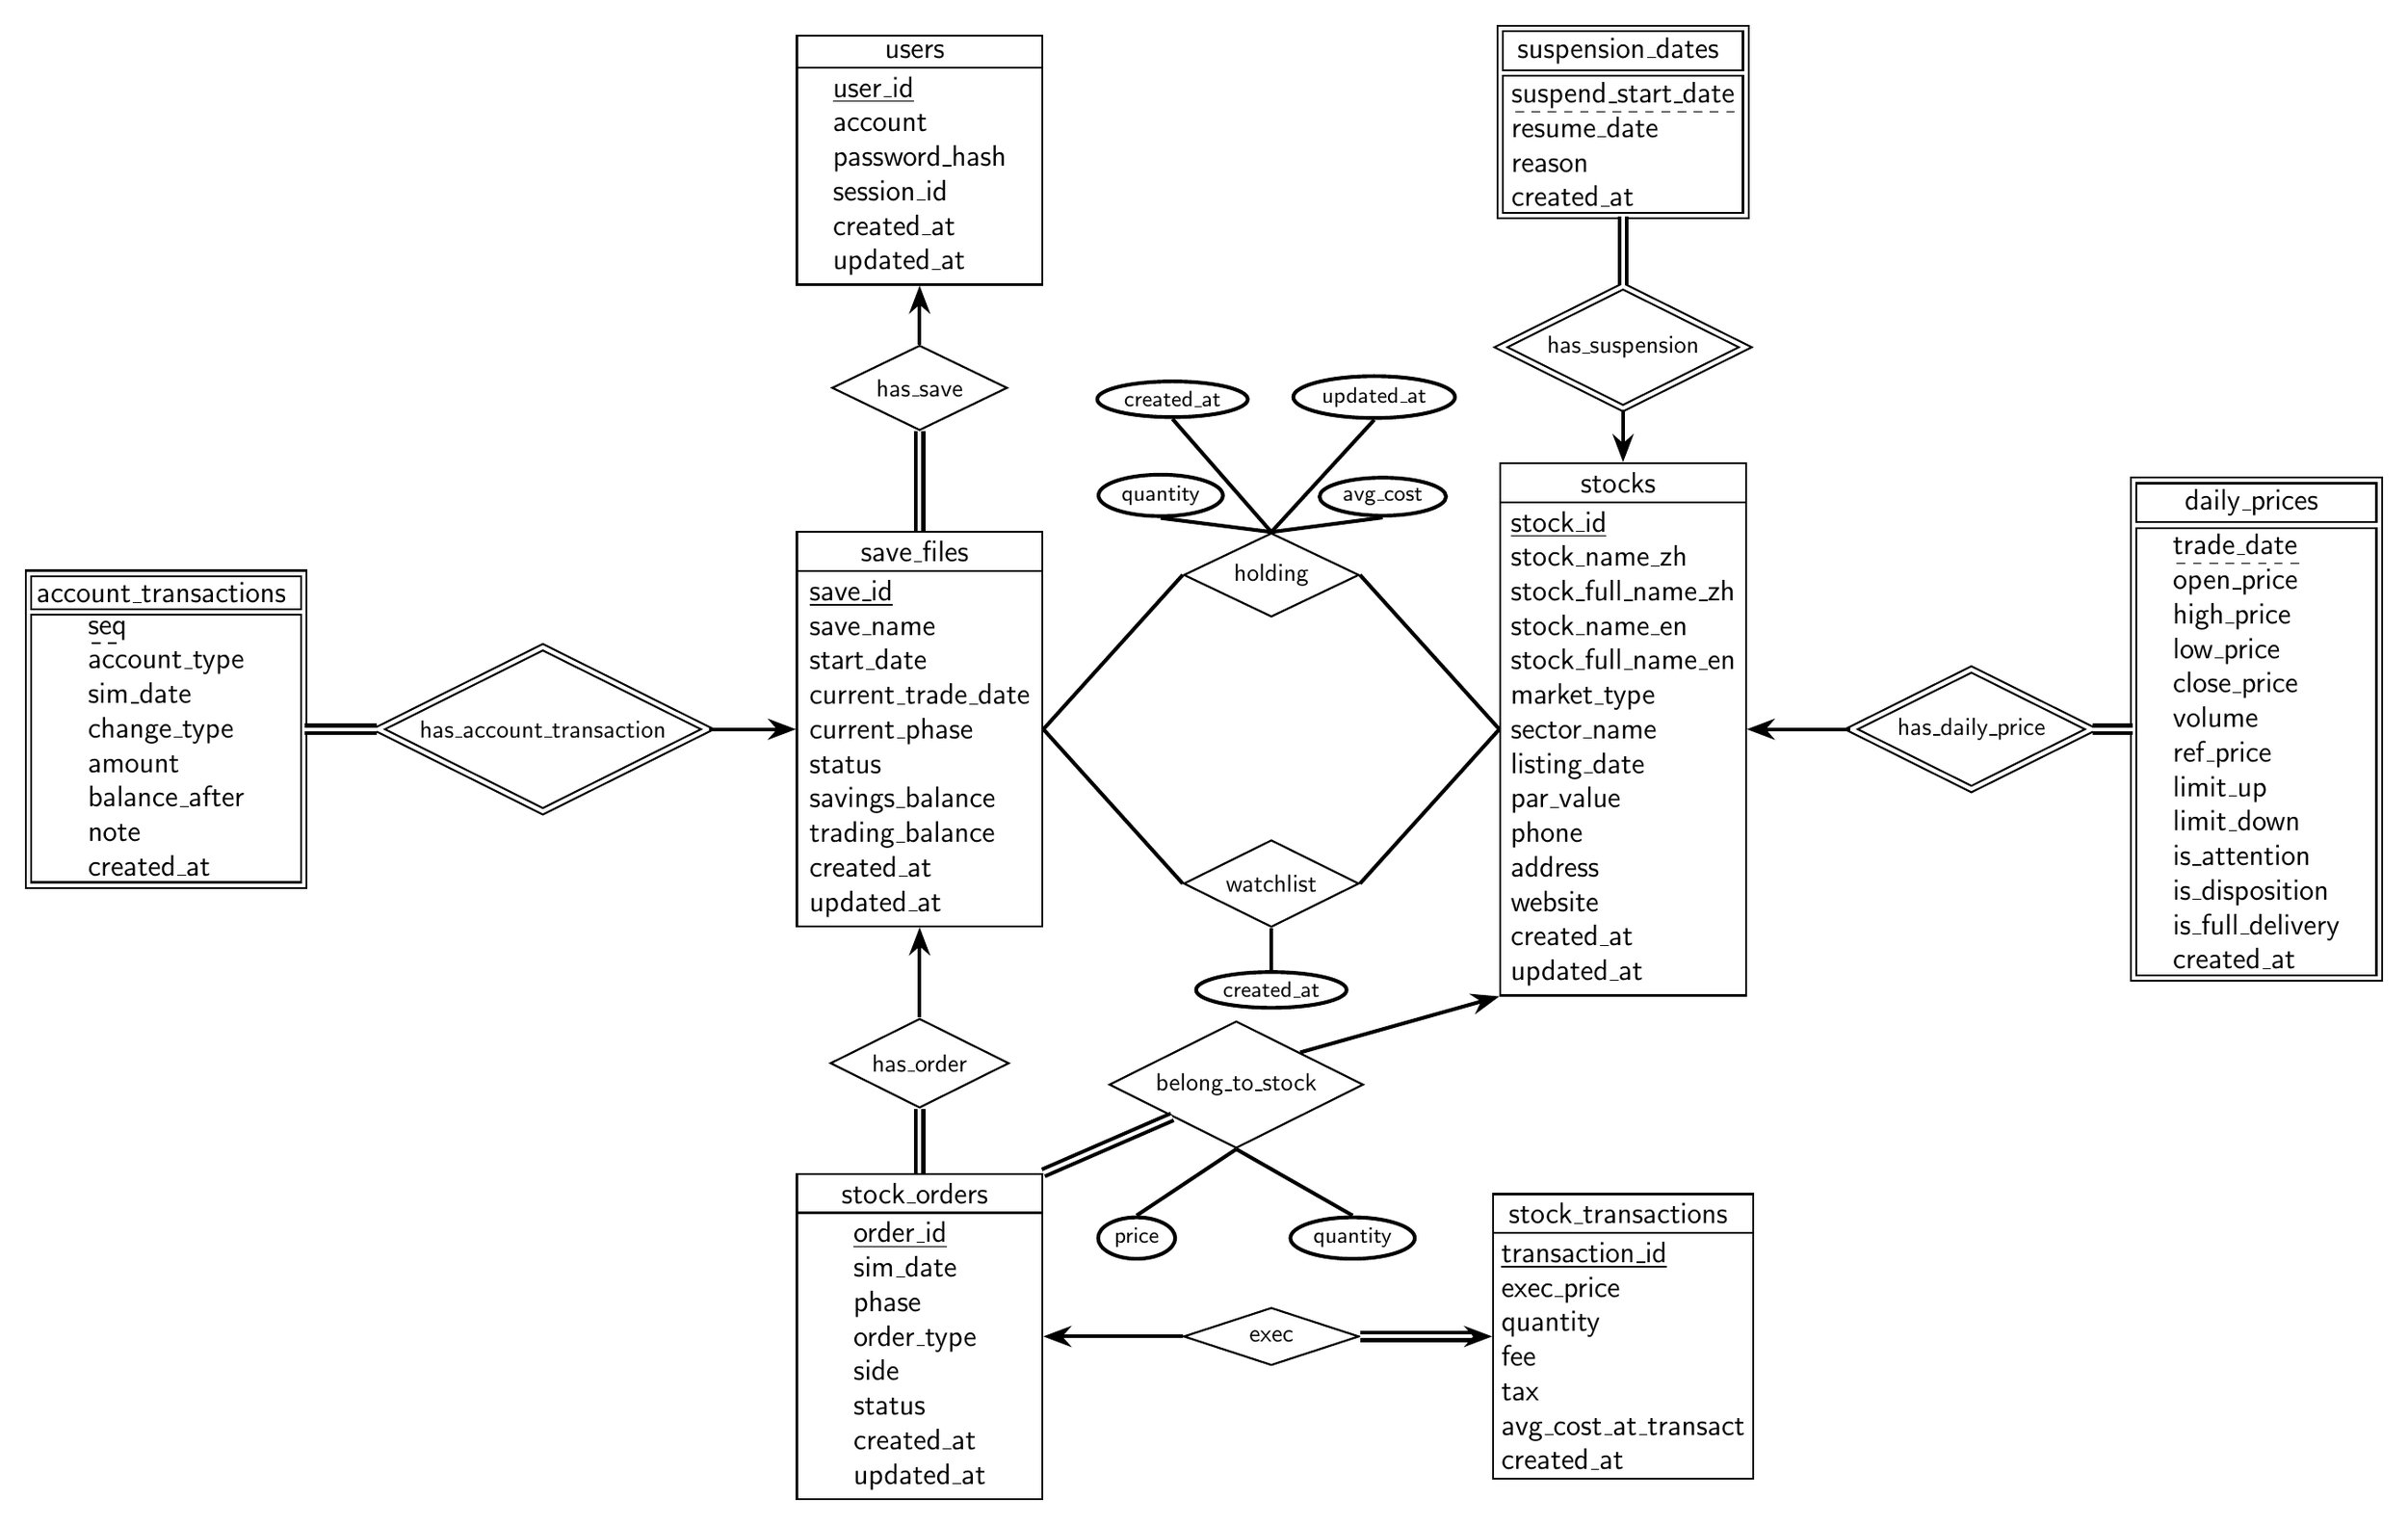
\begin{tikzpicture}[
        >={Stealth[length=4mm, width=3mm]},
        % >=stealth,
        % 線條樣式
        every path/.style={line width=1.5pt},
        % 實體樣式 (單線方框)
        entity/.style={
            rectangle split, rectangle split parts=2,
            draw, thick, align=left, minimum width=3.5cm, font=\sffamily\large
        },
        % 弱實體樣式 (雙線方框)
        weakentity/.style={
            rectangle split, rectangle split parts=2,
            draw, thick, double, double distance=1.5pt, align=left, minimum width=3.5cm, font=\sffamily\large
        },
        % 關聯樣式 (單線菱形)
        relationship/.style={
            diamond, draw, thick, aspect=2, minimum width=2.5cm, align=center, font=\sffamily
        },
        % 弱關聯樣式 (雙線菱形)
        weakrel/.style={
            diamond, draw, thick, double, double distance=1.5pt, aspect=2, minimum width=2.5cm, align=center, font=\sffamily
        },
        % 屬性樣式
        attribute/.style={
            ellipse, draw, align=center, font=\sffamily\small, inner sep=2pt
        },
        % 連線樣式 (全參與/雙線)
        total/.style={double, double distance=1.5pt} 
    ]

        % ==========================
        % 1. 建立實體 (Entities)
        % ==========================
        
        % SaveFile (中心)
        \node[entity] (savefile) {
            \hfil save\_files \hfil 
            \nodepart{two} 
            \underline{save\_id} \\ save\_name \\ start\_date \\ current\_trade\_date \\ 
            current\_phase \\ status \\ savings\_balance \\ trading\_balance \\ 
            created\_at \\ updated\_at
        };

        % User (上)
        \node[entity] (user) [above=3.5cm of savefile] {
            \hfil users \hfil 
            \nodepart{two} 
            \underline{user\_id} \\ account \\ password\_hash \\ session\_id \\
            created\_at \\ updated\_at
        };

        % AccountTransaction (左) - 弱實體
        \node[weakentity] (acctrans) [left=7cm of savefile] {
            \hfil account\_transactions \hfil 
            \nodepart{two} 
            \dashuline{seq} \\ account\_type \\ sim\_date \\ 
            change\_type \\ amount \\ balance\_after \\ note \\ created\_at
        };

        % Stock (右)
        \node[entity] (stock) [right=6.5cm of savefile] {
            \hfil stocks \hfil 
            \nodepart{two} 
            \underline{stock\_id} \\ stock\_name\_zh \\ stock\_full\_name\_zh \\ stock\_name\_en \\
            stock\_full\_name\_en \\ market\_type  \\ sector\_name  \\ 
            listing\_date \\ par\_value  \\ phone  \\ 
            address \\ website \\ created\_at \\ updated\_at
        };

        % DailyPrice (最右) - 弱實體
        \node[weakentity] (dailyprice) [right=5.5cm of stock] {
            \hfil daily\_prices \hfil 
            \nodepart{two} 
            \dashuline{trade\_date} \\ open\_price \\ high\_price \\ low\_price \\ close\_price \\ 
            volume \\ ref\_price \\ limit\_up \\ 
            limit\_down \\ is\_attention \\ 
            is\_disposition \\ is\_full\_delivery \\ created\_at
        };

        % SuspensionDate (上) - 弱實體 (依賴 Stock)
        \node[weakentity] (suspensiondate) [above=3.5cm of stock] {
            \hfil suspension\_dates \hfil 
            \nodepart{two} 
            \dashuline{suspend\_start\_date} \\ resume\_date \\ reason \\ created\_at
        };

        % StockOrder (下)
        \node[entity] (stockorder) [below=3.5cm of savefile] {
            \hfil stock\_orders \hfil 
            \nodepart{two} 
            \underline{order\_id} \\ sim\_date \\ phase \\ 
            order\_type  \\ side \\ status \\ 
            created\_at \\ updated\_at
        };

        % StockTransaction (StockOrder的右側，Stock的正下方)
        \node[entity] (stocktrans) at (stock |- stockorder) {
            \hfil stock\_transactions \hfil 
            \nodepart{two} 
            \underline{transaction\_id} \\ exec\_price \\ 
            quantity  \\ fee  \\ tax \\ 
            avg\_cost\_at\_transact \\ created\_at
        };

        % ==========================
        % 2. 建立關聯與連線
        % ==========================

        % User <-> SaveFile 
        \node[relationship] (hassave) at ($(user)!0.4!(savefile)$) {has\_save};
        \draw[<-] (user.south) -- (hassave.north);
        \draw[total] (savefile.north) -- (hassave.south);

        % SaveFile <-> AccountTransaction (弱關聯)
        \node[weakrel] (hasacctrans) at ($(savefile)!0.5!(acctrans)$) {has\_account\_transaction};
        \draw[<-] (savefile.west) -- (hasacctrans.east);
        \draw[total] (hasacctrans.west) -- (acctrans.east);

        % SaveFile <-> Stock (Holding & Watchlist)
        \path (savefile.east) -- (stock.west) coordinate[midway] (mid_ss);
        \node[relationship] (holding) at ($(mid_ss) + (0, 2.2)$) {holding};
        \node[relationship] (watchlist) at ($(mid_ss) + (0, -2.2)$) {watchlist};

        \draw (savefile.east) -- (holding.west);
        \draw (savefile.east) -- (watchlist.west);
        \draw (holding.east) -- (stock.west);
        \draw (watchlist.east) -- (stock.west);

        % Holding 屬性 (全部配置於上方並呈扇形展開)
        \node[attribute] (qty) [above left=0.6cm and 0.3cm of holding] {quantity};
        \node[attribute] (avgcost) [above right =0.6cm and 0.3cm of holding] {avg\_cost};
        \node[attribute] (h_created) [above left = 2cm and 0cm of holding] {created\_at};
        \node[attribute] (h_updated) [above right= 2cm and 0cm of holding] {updated\_at};
        
        % 全部將線條連接到 holding 的正上方 (north)
        \draw (holding.north) -- (qty.south);
        \draw (holding.north) -- (avgcost.south);
        \draw (holding.north) -- (h_created.south);
        \draw (holding.north) -- (h_updated.south);

        % Watchlist 屬性
        \node[attribute] (w_created) [below=0.6cm of watchlist] {created\_at};
        \draw (watchlist.south) -- (w_created.north);

        % Stock <-> DailyPrice (弱關聯)
        \node[weakrel] (hasdailyprice) at ($(stock)!0.55!(dailyprice)$) {has\_daily\_price};
        \draw[<-] (stock.east) -- (hasdailyprice.west);
        \draw[total] (hasdailyprice.east) -- (dailyprice.west);

        % Stock <-> SuspensionDate (弱關聯)
        \node[weakrel] (hassuspension) [above=0.75cm of stock.north] {has\_suspension};
        \draw[<-] (stock.north) -- (hassuspension.south);
        \draw[total] (hassuspension.north) -- (suspensiondate.south);

        % SaveFile <-> StockOrder
        \node[relationship] (hasorder) at ($(savefile)!0.55!(stockorder)$) {has\_order};
        \draw[<-] (savefile.south) -- (hasorder.north);
        \draw[total] (hasorder.south) -- (stockorder.north);

        % StockOrder <-> StockTransaction (exec)
        \node[relationship] (exec) at ($(stockorder)!0.5!(stocktrans)$) {exec};
        \draw[<-] (stockorder.east) -- (exec.west);
        \draw[total,->] (exec.east) -- (stocktrans.west);

        % StockOrder <-> Stock (belong_to_stock)
        % 將菱形置於兩者連線的中間偏左上角，避免線條與其他實體重疊
        \node[relationship] (belongto) at ($(stockorder.north east)!0.5!(stock.south west) + (-0.5, 0)$) {belong\_to\_stock};
        \draw[total] (stockorder.north east) -- (belongto.south west);
        \draw[<-] (stock.south west) -- (belongto.north east);

        \node[attribute] (b_price) [below left=1.5cm and 0.1cm of belongto] {price};
        \node[attribute] (b_qty) [below right=1.5cm and 0.1cm of belongto] {quantity};
        
        \draw (belongto.south) -- (b_price.north);
        \draw (belongto.south) -- (b_qty.north);
    \end{tikzpicture}
}
\end{center}

    \subsection{說明}
    \subsubsection{回應老師的提問}
        \begin{enumerate}
            \item price 與 quantity 的位置。\\
            我們同意老師的建議，將 price 與 quantity 從 StockOrder 的屬性改為 belong\_to\_stock 關聯的屬性，因為這兩個屬性是描述委託單與股票之間的關係，而非委託單本身的固有屬性。
            \item 如果一筆 transation 只有一個 stock 為何有 \verb|avg_cost_at_transact|？\\
            在此系統架構中，\verb|stock_orders|（委託單）與 \verb|stock_transactions|（股票交易紀錄）雖為 1 對 1 關聯，但兩者肩負的「業務職責」完全不同。
            \begin{itemize}
                \item \verb|stock_orders| 記錄的是「單次行為」：它只在乎「玩家在什麼時間，用多少錢（price）下單了多少張股票」。它是一張單純的收據。
                \item \verb|stock_transactions| 記錄的是「財務結果」：它必須承載會計結算的意義。
                在台股的「移動平均成本法」下，一筆「賣出」訂單的獲利，不能只看這張訂單本身，
                還必須參考過去所有買進訂單累積下來的平均成本。因此，\verb|avg_cost_at_transact| 
                負責補足持股（holding）所缺乏的「歷史持股成本」脈絡。
            \end{itemize}
            \verb|stock_transactions| 作為一個歷史紀錄用，以便之後欲開發回朔功能時更便於回朔。
        \end{enumerate}
    \subsection{修改}
        \subsubsection{修改 Table 命名規則}
        為了保持資料表命名的一致性與清晰性，我們將所有資料表的名稱統一改為複數形式，並使用底線分隔單字，以符合一般資料庫命名慣例。
        
        \subsubsection{欄位名稱}
        DailyPrice 的 open、high、low、close 欄位名稱修改為 open\_price、high\_price、low\_price、close\_price，以更明確的表達欄位內容。
        User 的 password 欄位名稱修改為 password\_hash，以強調該欄位存儲的是密碼的雜湊值，而非明文密碼。
        \subsubsection{新增時間戳記欄位}
        為了提升系統的維運追蹤能力、資料除錯效率，以及支援前端介面的功能展示，我們在所有資料表中全面導入了時間戳記（Timestamp）欄位。依據資料的生命週期與變動特性，具體的設計邏輯分為以下兩類：
        
        \begin{itemize}
            \item \textbf{狀態會變動的資料表（新增 \texttt{created\_at} 與 \texttt{updated\_at}）}：
            
            針對資料建立後，其內容或狀態會隨著業務邏輯持續更新的實體，例如 \verb|users|、\verb|stocks|、\verb|save_files|、\verb|stock_orders| 與 \verb|holdings|。這能幫助系統精確掌握資料的初始化時間與最後一次修改時間（例如追蹤一筆委託單狀態從 PENDING 轉為 FILLED 的時間點）。
            
            \item \textbf{歷史紀錄與狀態單一的資料表（僅新增 \texttt{created\_at}）：}
            
            針對屬於唯讀日誌性質，或者只有「新增／刪除」而沒有「修改」行為的資料表，我們僅保留建立時間以節省空間。
            此類包含 \verb|account_transactions|、\verb|daily_prices|、\verb|stock_transactions|、\verb|suspension_dates| 以及 \verb|watchlists|。
            
        \end{itemize}
        \subsubsection{欄位名稱與保留字相同之修正}
        在 \verb|save_files| 表中，將 \verb|current_date| 欄位名稱修改為 \verb|current_trade_date|，以避免與 SQL 保留字 \verb|CURRENT_DATE| 發生衝突，並更明確地表達該欄位的用途。
    \section{E-R diagram 轉成 Relational Table 之 DDL 的形式}
    \subsection{使用者憑證表 (users)}
    \lstinputlisting[language=SQL, firstline=21, lastline=31]{../schema/ddl.sql}

    此資料表負責儲存玩家登入帳戶的憑證與登入狀態資訊，用以進行身分驗證與單一登入防呆。

    \begin{center}
    \begin{tabular}{|l|l|p{8cm}|}
    \hline
    \textbf{欄位名稱} & \textbf{資料型態} & \textbf{欄位說明} \\ \hline
    user\_id & BIGINT UNSIGNED & 使用者唯一識別碼 (Primary Key，自動遞增) \\ \hline
    account & VARCHAR(50) & 登入帳號 (Unique Key) \\ \hline
    password\_hash & VARCHAR(255) & 密碼的安全雜湊值 (防範明碼外洩) \\ \hline
    session\_id & CHAR(36) & 登入狀態憑證 Token (Unique Key，防範異地登入) \\ \hline
    created\_at & TIMESTAMP & 帳戶註冊建立時間 \\ \hline
    updated\_at & TIMESTAMP & 帳戶狀態最後更新時間 \\ \hline
    \end{tabular}
    \end{center}

    \subsubsection*{外鍵與約束限制 (Constraints)}
    \begin{itemize}
        \item \textbf{PRIMARY KEY}：\texttt{user\_id}。
        \item \textbf{UNIQUE KEY}：
            \begin{itemize}
                \item \texttt{uq\_users\_account} (\texttt{account})：確保帳號不重複。
                \item \texttt{uq\_users\_session\_id} (\texttt{session\_id})：確保同一時間只有一處登入憑證有效（單一登入原則，允許為 \texttt{NULL}）。
            \end{itemize}
    \end{itemize}

    \subsection{股票基本面表 (stocks)}
    \lstinputlisting[language=SQL, firstline=33, lastline=51]{../schema/ddl.sql}

    此資料表儲存台股各檔股票與指數之靜態基本面資訊，作為唯讀的字典檔。其上市日期 \texttt{listing\_date} 亦提供進行交易日期的上市資格校驗。
    \vspace{-0.5cm}
    \begin{center}
    \begin{tabular}{|l|l|p{8cm}|}
    \hline
    \textbf{欄位名稱} & \textbf{資料型態} & \textbf{欄位說明} \\ \hline
    stock\_id & VARCHAR(16) & 股票或指數代碼 (Primary Key，如 2330) \\ \hline
    stock\_name\_zh & VARCHAR(64) & 中文簡稱 (如 台積電) \\ \hline
    stock\_full\_name\_zh & VARCHAR(128) & 中文全名 (如 台灣積體電路製造) \\ \hline
    stock\_name\_en & VARCHAR(64) & 英文簡稱 (可為 NULL) \\ \hline
    stock\_full\_name\_en & VARCHAR(128) & 英文全名 (可為 NULL) \\ \hline
    market\_type & ENUM(...) & 市場別 (TSE: 上市, OTC: 上櫃, EMERGING: 興櫃, INDEX: 指數) \\ \hline
    sector\_name & VARCHAR(64) & 產業類別名稱 (如 半導體業，可為 NULL) \\ \hline
    listing\_date & DATE & 最近一次上市/發行日期 (可為 NULL) \\ \hline
    par\_value & DECIMAL(10, 2) & 股票每股面額 (如 10.00，可為 NULL) \\ \hline
    phone & VARCHAR(32) & 公司聯絡電話 (可為 NULL) \\ \hline
    address & VARCHAR(255) & 公司地址 (可為 NULL) \\ \hline
    website & VARCHAR(255) & 公司官方網站 URL (可為 NULL) \\ \hline
    created\_at & TIMESTAMP & 欄位建立時間 \\ \hline
    updated\_at & TIMESTAMP & 欄位最後更新時間 \\ \hline
    \end{tabular}
    \end{center}
    % \footnotetext{本系統僅先儲存上市 (TSE) 與指數 (INDEX) 資料。}

    \subsubsection*{外鍵與約束限制 (Constraints)}
    \begin{itemize}
        \item \textbf{PRIMARY KEY}：\texttt{stock\_id}。
        \item \textbf{INDEX}：
            \begin{itemize}
                \item \texttt{idx\_stocks\_market\_type} (\texttt{market\_type})：加速依市場類型篩選股票之查詢。
                \item \texttt{idx\_stocks\_sector\_name} (\texttt{sector\_name})：加速依產業篩選股票之查詢。
            \end{itemize}
    \end{itemize}

    \subsection{歷史日線行情表 (daily\_prices)}
    \lstinputlisting[language=SQL, firstline=53, lastline=92]{../schema/ddl.sql}

    此資料表儲存每檔股票或指數在每個交易日的開盤、最高、最低、收盤價格與成交量等行情，為交易撮合與 K 線圖繪製之核心依據。

    \begin{center}
    \begin{tabular}{|l|l|p{8cm}|}
    \hline
    \textbf{欄位名稱} & \textbf{資料型態} & \textbf{欄位說明} \\ \hline
    stock\_id & VARCHAR(16) & 股票或指數代碼 (Primary Key，Foreign Key) \\ \hline
    trade\_date & DATE & 交易日期 (Primary Key) \\ \hline
    open\_price & DECIMAL(10, 2) & 今日開盤價 \\ \hline
    high\_price & DECIMAL(10, 2) & 今日最高價 \\ \hline
    low\_price & DECIMAL(10, 2) & 今日最低價 \\ \hline
    close\_price & DECIMAL(10, 2) & 今日收盤價 \\ \hline
    volume & BIGINT UNSIGNED & 當日成交量 (單位：股) \\ \hline
    ref\_price & DECIMAL(10, 2) & 當日開盤參考價 (可為 NULL) \\ \hline
    limit\_up & DECIMAL(10, 2) & 當日漲停價 (可為 NULL) \\ \hline
    limit\_down & DECIMAL(10, 2) & 當日跌停價 (可為 NULL) \\ \hline
    is\_attention & BOOLEAN & 是否為注意股 (預設為 FALSE) \\ \hline
    is\_disposition & BOOLEAN & 是否為處置股 (預設為 FALSE) \\ \hline
    is\_full\_delivery & BOOLEAN & 是否為全額交割股 (預設為 FALSE) \\ \hline
    created\_at & TIMESTAMP & 欄位建立時間 \\ \hline
    \end{tabular}
    \end{center}

    \subsubsection*{外鍵與約束限制 (Constraints)}
    \begin{itemize}
        \item \textbf{PRIMARY KEY}：\texttt{(stock\_id, trade\_date)}。
        \item \textbf{FOREIGN KEY}：
            \begin{itemize}
                \item \texttt{fk\_daily\_prices\_stock}：\texttt{stock\_id} 參考 \texttt{stocks(stock\_id)}，採 \texttt{ON UPDATE CASCADE ON DELETE RESTRICT} 以維護關聯完整性。
            \end{itemize}
        \item \textbf{INDEX}：
            \begin{itemize}
                \item \texttt{idx\_daily\_prices\_trade\_date} (\texttt{trade\_date})：加速跨股票查詢特定交易日報價之效能。
            \end{itemize}
        \item \textbf{CHECK}：
            \begin{itemize}
                \item \texttt{chk\_daily\_prices\_price\_range}：確保所有價格欄位均為非負數，且滿足合理價格區間限制（最低價 $\le$ 開/收/最高價，最高價 $\ge$ 開/收價，以及漲停價 $\ge$ 跌停價）。
                \item \texttt{chk\_daily\_prices\_non\_negative\_volume}：確保成交量大於或等於 0。
            \end{itemize}
    \end{itemize}

    \subsection{暫停交易日期表 (suspension\_dates)}
    \lstinputlisting[language=SQL, firstline=94, lastline=108]{../schema/ddl.sql}
    \begin{center}
    \begin{tabular}{|l|l|p{8cm}|}
    \hline
    \textbf{欄位名稱} & \textbf{資料型態} & \textbf{欄位說明} \\ \hline
    stock\_id & VARCHAR(16) & 股票代碼 (Primary Key，Foreign Key) \\ \hline
    suspend\_start\_date & DATE & 暫停交易開始日期 (Primary Key) \\ \hline
    resume\_date & DATE & 恢復交易日期 (可為 NULL，代表尚未復牌或為指數型商品) \\ \hline
    reason & VARCHAR(255) & 暫停交易原因 (如減資、颱風天、重大訊息等) \\ \hline
    created\_at & TIMESTAMP & 欄位建立時間 \\ \hline
    \end{tabular}
    \end{center}

    \subsubsection*{外鍵與約束限制 (Constraints)}
    \begin{itemize}
        \item \textbf{PRIMARY KEY}：\texttt{(stock\_id, suspend\_start\_date)}。
        \item \textbf{FOREIGN KEY}：
            \begin{itemize}
                \item \texttt{fk\_suspension\_dates\_stock}：\texttt{stock\_id} 參考 \texttt{stocks(stock\_id)}，採 \texttt{ON UPDATE CASCADE ON DELETE RESTRICT}。
            \end{itemize}
        \item \textbf{INDEX}：
            \begin{itemize}
                \item \texttt{idx\_suspension\_dates\_resume\_date} (\texttt{resume\_date})：加速篩選並查詢已復牌股票之效能。
            \end{itemize}
        \item \textbf{CHECK}：
            \begin{itemize}
                \item \texttt{chk\_suspension\_dates\_order}：確保復牌日期大於或等於停牌開始日期\\（\texttt{resume\_date >= suspend\_start\_date}，若為 \texttt{NULL} 則不限）。
            \end{itemize}
    \end{itemize}

    \subsection{模擬存檔表 (save\_files)}
    \lstinputlisting[language=SQL, firstline=110, lastline=135]{../schema/ddl.sql}

    此資料表作為模擬系統的核心狀態機，負責控管個別玩家的模擬進度、虛擬時間軸、當前交易階段與雙帳戶餘額。

    \begin{center}
    \begin{tabular}{|l|l|p{8cm}|}
    \hline
    \textbf{欄位名稱} & \textbf{資料型態} & \textbf{欄位說明} \\ \hline
    save\_id & BIGINT UNSIGNED & 存檔唯一識別碼 (Primary Key，自動遞增) \\ \hline
    user\_id & BIGINT UNSIGNED & 所屬玩家識別碼 (Foreign Key) \\ \hline
    save\_name & VARCHAR(100) & 存檔自訂名稱 \\ \hline
    start\_date & DATE & 時光機模擬初始歷史日期 \\ \hline
    current\_trade\_date & DATE & 當前虛擬交易日期 \\ \hline
    current\_phase & ENUM(...) & 當前交易階段 (PRE\_MARKET, INTRADAY, POST\_MARKET, CLOSED) \\ \hline
    status & ENUM(...) & 存檔生命週期狀態 (ACTIVE, BANKRUPT, FINISHED) \\ \hline
    savings\_balance & DECIMAL(18, 2) & 存款戶餘額 (預設為 0.00) \\ \hline
    trading\_balance & DECIMAL(18, 2) & 交割戶餘額 (預設為 0.00) \\ \hline
    created\_at & TIMESTAMP & 存檔建立時間 \\ \hline
    updated\_at & TIMESTAMP & 存檔狀態最後更新時間 \\ \hline
    \end{tabular}
    \end{center}

    \subsubsection*{外鍵與約束限制 (Constraints)}
    \begin{itemize}
        \item \textbf{PRIMARY KEY}：\texttt{save\_id}。
        \item \textbf{UNIQUE KEY}：
            \begin{itemize}
                \item \texttt{uq\_save\_files\_user\_save\_name} (\texttt{user\_id, save\_name})：確保同一個玩家無法建立同名的模擬存檔。
            \end{itemize}
        \item \textbf{FOREIGN KEY}：
            \begin{itemize}
                \item \texttt{fk\_save\_files\_user}：\texttt{user\_id} 參考 \texttt{users(user\_id)}，\\採 \texttt{ON UPDATE CASCADE ON DELETE RESTRICT}。
            \end{itemize}
        \item \textbf{INDEX}：
            \begin{itemize}
                \item \texttt{idx\_save\_files\_user\_id} (\texttt{user\_id})：加速查詢特定玩家的所有存檔。
                \item \texttt{idx\_save\_files\_user\_status} (\texttt{user\_id, status})：加速查詢與計算玩家目前進行中的存檔數量。
                \item \texttt{idx\_save\_files\_status} (\texttt{status})：加速依存檔狀態進行全局數據統計。
            \end{itemize}
        \item \textbf{CHECK}：
            \begin{itemize}
                \item \texttt{chk\_save\_files\_balances}：確保存款戶與交割戶之餘額皆大於或等於 0，避免產生非法的負餘額。
                \item \texttt{chk\_save\_files\_dates}：確保當前虛擬交易日期大於或等於初始歷史日期（\texttt{current\_trade\_date >= start\_date}）。
            \end{itemize}
    \end{itemize}

    \subsection{帳戶金流明細表 (account\_transactions)}
    \lstinputlisting[language=SQL, firstline=137, lastline=160]{../schema/ddl.sql}

    此資料表採用會計流水帳的概念，完整記錄玩家模擬存檔中存款戶與交割戶的每一筆資金異動軌跡，用以進行歷史金流追蹤與繪製資產曲線。

    \begin{center}
    \begin{tabular}{|l|l|p{8cm}|}
    \hline
    \textbf{欄位名稱} & \textbf{資料型態} & \textbf{欄位說明} \\ \hline
    save\_id & BIGINT UNSIGNED & 所屬存檔識別碼 (Primary Key，Foreign Key) \\ \hline
    seq & INT UNSIGNED & 存檔內明細流水號 (Primary Key，由 1 開始遞增) \\ \hline
    account\_type & ENUM(...) & 帳戶類型 (SAVINGS: 存款戶, TRADING: 交割戶) \\ \hline
    sim\_date & DATE & 金流發生的虛擬日期 \\ \hline
    change\_type & VARCHAR(50) & 異動類型 (如資金轉帳、交易扣款、交易入帳等) \\ \hline
    amount & DECIMAL(18, 2) & 金流異動金額 \\ \hline
    balance\_after & DECIMAL(18, 2) & 異動後之帳戶餘額快照 \\ \hline
    note & VARCHAR(255) & 額外備註說明 (可為 NULL) \\ \hline
    created\_at & TIMESTAMP & 明細記錄建立時間 \\ \hline
    \end{tabular}
    \end{center}

    \subsubsection*{外鍵與約束限制 (Constraints)}
    \begin{itemize}
        \item \textbf{PRIMARY KEY}：\texttt{(save\_id, seq)}。
        \item \textbf{FOREIGN KEY}：
            \begin{itemize}
                \item \texttt{fk\_account\_transactions\_save}：\texttt{save\_id} 參考 \texttt{save\_files(save\_id)}，\\採 \texttt{ON UPDATE CASCADE ON DELETE CASCADE}，確保存存檔刪除時明細同步清除。
            \end{itemize}
        \item \textbf{INDEX}：
            \begin{itemize}
                \item \texttt{idx\_account\_transactions\_sim\_date} (\texttt{sim\_date})：加速特定模擬日期之金流明細查詢。
                \item \texttt{idx\_account\_transactions\_change\_type} (\texttt{change\_type})：加速特定交易類型的查詢。
            \end{itemize}
        \item \textbf{CHECK}：
            \begin{itemize}
                \item \texttt{chk\_account\_transactions\_seq}：確保流水號 \texttt{seq} 大於 0。
                \item \texttt{chk\_account\_transactions\_amount}：確保異動金額大於或等於 0。
                \item \texttt{chk\_account\_transactions\_balance\_after}：確保異動後之餘額快照大於或等於 0。
            \end{itemize}
    \end{itemize}

    \subsection{股票委託單表 (stock\_orders)}
    \lstinputlisting[language=SQL, firstline=162, lastline=195]{../schema/ddl.sql}

    此資料表記錄玩家在特定模擬存檔中發出的買賣委託單，包含限價單、市價單與定價委託，為撮合引擎的運算對象。

    \begin{center}
    \begin{tabular}{|l|l|p{8cm}|}
    \hline
    \textbf{欄位名稱} & \textbf{資料型態} & \textbf{欄位說明} \\ \hline
    order\_id & BIGINT UNSIGNED & 委託單唯一識別碼 (Primary Key，自動遞增) \\ \hline
    save\_id & BIGINT UNSIGNED & 所屬存檔識別碼 (Foreign Key) \\ \hline
    stock\_id & VARCHAR(16) & 委託標的代碼 (Foreign Key) \\ \hline
    sim\_date & DATE & 委託時的虛擬日期 \\ \hline
    phase & ENUM(...) & 委託交易階段 (PRE\_MARKET, INTRADAY, POST\_MARKET) \\ \hline
    order\_type & ENUM(...) & 委託類型 (LIMIT: 限價單, MARKET: 市價單) \\ \hline
    side & ENUM(...) & 買賣方向 (BUY: 買進, SELL: 賣出) \\ \hline
    price & DECIMAL(10, 2) & 限價單之指定價格 (市價單則為 NULL) \\ \hline
    quantity & INT UNSIGNED & 委託股數 (單位：股，下單最小限制為 1000 股) \\ \hline
    status & ENUM(...) & 委託單狀態 (PENDING: 待撮合, FILLED: 已成交, CANCELED: 撤單, EXPIRED: 逾期失效, REJECTED: 拒絕下單) \\ \hline
    created\_at & TIMESTAMP & 委託單建立時間 \\ \hline
    updated\_at & TIMESTAMP & 委託單狀態最後更新時間 \\ \hline
    \end{tabular}
    \end{center}

    \subsubsection*{外鍵與約束限制 (Constraints)}
    \begin{itemize}
        \item \textbf{PRIMARY KEY}：\texttt{order\_id}。
        \item \textbf{FOREIGN KEY}：
            \begin{itemize}
                \item \texttt{fk\_stock\_orders\_save}：\texttt{save\_id} 參考 \texttt{save\_files(save\_id)}，\\採 \texttt{ON UPDATE CASCADE ON DELETE CASCADE}。
                \item \texttt{fk\_stock\_orders\_stock}：\texttt{stock\_id} 參考 \texttt{stocks(stock\_id)}，\\採 \texttt{ON UPDATE CASCADE ON DELETE RESTRICT}。
            \end{itemize}
        \item \textbf{INDEX}：
            \begin{itemize}
                \item \texttt{idx\_stock\_orders\_save\_id} (\texttt{save\_id})：加速查詢特定存檔的委託單。
                \item \texttt{idx\_stock\_orders\_stock\_id} (\texttt{stock\_id})：加速查詢特定股票的委託紀錄。
                \item \texttt{idx\_stock\_orders\_sim\_date} (\texttt{sim\_date})：加速依模擬日期篩選委託單。
                \item \texttt{idx\_stock\_orders\_status} (\texttt{status})：加速篩選未成交或已成交的委託單以進行撮合。
            \end{itemize}
        \item \textbf{CHECK}：
            \begin{itemize}
                \item \texttt{chk\_stock\_orders\_quantity}：確保委託股數大於 0。
                \item \texttt{chk\_stock\_orders\_price}：確保限價單必須指定大於 0 的價格；市價單之價格欄位必須為空值 (\texttt{NULL})。
            \end{itemize}
    \end{itemize}

    \subsection{股票交易紀錄表 (stock\_transactions)}
    \lstinputlisting[language=SQL, firstline=197, lastline=217]{../schema/ddl.sql}
    \begin{center}
    \begin{tabular}{|l|l|p{6cm}|}
    \hline
    \textbf{欄位名稱} & \textbf{資料型態} & \textbf{欄位說明} \\ \hline
    transaction\_id & BIGINT UNSIGNED & 交易明細唯一識別碼 (Primary Key，自動遞增) \\ \hline
    order\_id & BIGINT UNSIGNED & 對應之委託單識別碼 (Unique Key，Foreign Key) \\ \hline
    exec\_price & DECIMAL(10, 2) & 實際成交單價 \\ \hline
    quantity & INT UNSIGNED & 成交股數 (單位：股) \\ \hline
    fee & DECIMAL(10, 2) & 券商交易手續費 (買賣雙向收取，最低 20 元) \\ \hline
    tax & DECIMAL(10, 2) & 國家證券交易稅 (僅在賣出時收取，稅率 0.3\%) \\ \hline
    avg\_cost\_at\_transact & DECIMAL(10, 4) & 成交當下的持股平均成本快照 (可為 NULL) \\ \hline
    created\_at & TIMESTAMP & 交易紀錄建立時間 \\ \hline
    \end{tabular}
    \end{center}

    \subsubsection*{外鍵與約束限制 (Constraints)}
    \begin{itemize}
        \item \textbf{PRIMARY KEY}：\texttt{transaction\_id}。
        \item \textbf{UNIQUE KEY}：
            \begin{itemize}
                \item \texttt{uq\_stock\_transactions\_order\_id} (\texttt{order\_id})：確保一筆委託單至多只會對應一筆成交明細，落實 1 對 1 關係。
            \end{itemize}
        \item \textbf{FOREIGN KEY}：
            \begin{itemize}
                \item \texttt{fk\_stock\_transactions\_order}：\texttt{order\_id} 參考 \texttt{stock\_orders(order\_id)}，\\採 \texttt{ON UPDATE CASCADE ON DELETE CASCADE}。
            \end{itemize}
        \item \textbf{CHECK}：
            \begin{itemize}
                \item \texttt{chk\_stock\_transactions\_quantity}：確保成交股數大於 0。
                \item \texttt{chk\_stock\_transactions\_amounts}：確保成交單價大於 0，手續費、證交稅均大於或等於 0，且若平均成本快照不為空值，則其必須大於或等於 0。
            \end{itemize}
    \end{itemize}

    \subsection{持股表 (holdings)}
    \lstinputlisting[language=SQL, firstline=218, lastline=237]{../schema/ddl.sql}

    此資料表作為多對多之中介表，用以追蹤玩家在各模擬存檔中的股票庫存數量與加權平均成本，為計算帳面市值與未實現損益的核心來源。

    \begin{center}
    \begin{tabular}{|l|l|p{8cm}|}
    \hline
    \textbf{欄位名稱} & \textbf{資料型態} & \textbf{欄位說明} \\ \hline
    save\_id & BIGINT UNSIGNED & 所屬存檔識別碼 (Primary Key，Foreign Key) \\ \hline
    stock\_id & VARCHAR(16) & 持有標的代碼 (Primary Key，Foreign Key) \\ \hline
    quantity & INT UNSIGNED & 持有股數 (單位：股，隨成交動態增減) \\ \hline
    avg\_cost & DECIMAL(10, 4) & 加權平均成本 (單位：元/股，含交易手續費攤平) \\ \hline
    created\_at & TIMESTAMP & 庫存欄位建立時間 \\ \hline
    updated\_at & TIMESTAMP & 庫存數量與成本最後更新時間 \\ \hline
    \end{tabular}
    \end{center}

    \subsubsection*{外鍵與約束限制 (Constraints)}
    \begin{itemize}
        \item \textbf{PRIMARY KEY}：\texttt{(save\_id, stock\_id)}。
        \item \textbf{FOREIGN KEY}：
            \begin{itemize}
                \item \texttt{fk\_holdings\_save}：\texttt{save\_id} 參考 \texttt{save\_files(save\_id)}，\\採 \texttt{ON UPDATE CASCADE ON DELETE CASCADE}。
                \item \texttt{fk\_holdings\_stock}：\texttt{stock\_id} 參考 \texttt{stocks(stock\_id)}，\\採 \texttt{ON UPDATE CASCADE ON DELETE RESTRICT}。
            \end{itemize}
        \item \textbf{INDEX}：
            \begin{itemize}
                \item \texttt{idx\_holdings\_stock\_id} (\texttt{stock\_id})：加速跨存檔查詢某檔股票的全局持有分布。
            \end{itemize}
        \item \textbf{CHECK}：
            \begin{itemize}
                \item \texttt{chk\_holdings\_values}：確保持有股數 \texttt{quantity} 與平均成本 \texttt{avg\_cost} 均大於或等於 0。
            \end{itemize}
    \end{itemize}

    \subsection{自選股表 (watchlists)}
    \lstinputlisting[language=SQL, firstline=239, lastline=253]{../schema/ddl.sql}

    此資料表作為多對多之中介表，用以追蹤玩家在各模擬存檔中自選關注的股票清單，確保跨存檔自選清單的完全隔離。

    \begin{center}
    \begin{tabular}{|l|l|p{8cm}|}
    \hline
    \textbf{欄位名稱} & \textbf{資料型態} & \textbf{欄位說明} \\ \hline
    save\_id & BIGINT UNSIGNED & 所屬存檔識別碼 (Primary Key，Foreign Key) \\ \hline
    stock\_id & VARCHAR(16) & 自選關注之股票代碼 (Primary Key，Foreign Key) \\ \hline
    created\_at & TIMESTAMP & 加入自選清單時間 \\ \hline
    \end{tabular}
    \end{center}

    \subsubsection*{外鍵與約束限制 (Constraints)}
    \begin{itemize}
        \item \textbf{PRIMARY KEY}：\texttt{(save\_id, stock\_id)}。
        \item \textbf{FOREIGN KEY}：
            \begin{itemize}
                \item \texttt{fk\_watchlists\_save}：\texttt{save\_id} 參考 \texttt{save\_files(save\_id)}，\\採 \texttt{ON UPDATE CASCADE ON DELETE CASCADE}。
                \item \texttt{fk\_watchlists\_stock}：\texttt{stock\_id} 參考 \texttt{stocks(stock\_id)}，\\採 \texttt{ON UPDATE CASCADE ON DELETE RESTRICT}。
            \end{itemize}
        \item \textbf{INDEX}：
            \begin{itemize}
                \item \texttt{idx\_watchlists\_stock\_id} (\texttt{stock\_id})：加速跨存檔查詢某檔股票被自選追蹤之次數。
            \end{itemize}
        \item \textbf{TRIGGER 約束}：
            \begin{itemize}
                \item 設有 \texttt{trg\_watchlists\_before\_insert} 觸發器，限制每個存檔最多只能加入 100 筆自選股。
            \end{itemize}
    \end{itemize}

    \section{系統內容功能詳細敘述}
    
    本模擬系統旨在建立一個高度擬真的台灣股市交易沙盒環境。為了使系統兼顧遊玩趣味性與金融交易的嚴謹性，系統功能圍繞於「玩家帳戶管理」、「模擬存檔隔離」、「時光機時間軸控制」、「銀行雙帳戶資產分配」、「盤面行情與技術指標查詢」、「撮合引擎邏輯」以及「持股與損益結算」等七個核心模組。

    \subsection{系統核心功能模組}
    \begin{enumerate}
        \item \textbf{帳戶登入與安全驗證}\\
        系統為單人模擬器，使用者需先進行註冊與登入。資料庫使用 Bcrypt 演算法安全儲存密碼。此外，為了防範 Race Condition，採用了單一登入 (SSO) 原則：使用者登入後，系統會生成一個安全登入憑證並寫入 \texttt{session\_id}，若同帳號於其他瀏覽器再次登入，新憑證將會覆蓋舊有憑證，使舊登入狀態失效。
        
        \item \textbf{多重模擬存檔管理} \\       
        每位使用者可同時建立並管理多個模擬存檔（時光沙盒），每個存檔的時間軸、資產餘額、持股庫存、自選股以及交易紀錄完全獨立，互不干涉。
        \begin{itemize}
            \item \textbf{進行中存檔上限}：每位玩家最多可同時擁有 5 個進行中 (\texttt{ACTIVE}) 存檔。
            \item \textbf{總存檔上限}：包含進行中、已破產 (\texttt{BANKRUPT}) 與手動結束封存 (\texttt{FINISHED})，\\每位玩家上限為 10 個。
            \item \textbf{防呆限制}：同一玩家帳戶下不可建立同名的模擬存檔。
        \end{itemize}

        \item \textbf{時間軸控制與資訊隔離}\\
        系統以「交易日」為基本時間單位。使用者可自由選擇歷史起點日期（或由系統隨機抽取），並手動點擊推進時間。
        每個交易日依序切換四個交易階段：\texttt{盤前} $\to$ \texttt{盤中} $\to$ \texttt{盤後} $\to$ \texttt{收市}。
        
        時光機引導之歷史資料揭露需嚴格遵守「時空隔離」原則，玩家僅能查詢當前虛擬日期以前已揭露之 K 線與價格，未推進到的日期或當日未收盤的資訊不得提前顯示，以徹底杜絕未來套利。

        \item \textbf{銀行系統與雙帳戶資產分配}\\
        為模擬真實的證券交易扣款，系統提供雙帳戶機制：
        \begin{itemize}
            \item \textbf{存款戶}：用於存放玩家暫不投入股票市場之銀行本金。
            \item \textbf{交割戶}：專門用於股票買賣成交時的款項交割與證券稅費扣收。
            \item 兩帳戶之間可即時互轉資金，不收任何費用。在正常狀態下，兩帳戶的餘額皆大於或等於 0，交割戶扣款不足即代表模擬破產。
        \end{itemize}

        \item \textbf{股票查詢與自選股管理}\\
        使用者可透過搜尋或市場類別瀏覽股票，並檢視歷史日 K、週 K、月 K 線圖與同週期的成交量圖。玩家可自由疊加常見技術指標。自選股清單隸屬於個別存檔，上限為 100 筆，且同一存檔內同檔股票不可重複加入。

        \item \textbf{交易規則限制}
        \begin{itemize}
            \item \textbf{整股交易}：所有委託買賣皆以整股（最低 1000 股）為單位，不接受零股交易。
            \item \textbf{不支援部分成交}：撮合結果僅有全部成交 (\texttt{FILLED}) 或全部不成交 (\texttt{EXPIRED}) 兩種。
            \item \textbf{無放空機制}：本版本不支援融資融券，且送出賣單時系統會先扣除當前階段所有 Pending 賣單，嚴格禁止超額賣出。
            \item \textbf{交易稅費}：買進手續費 0.1425\%；賣出手續費 0.1425\%，另收證券交易稅 0.3\%（單筆手續費不足 20 元以 20 元計）。
        \end{itemize}

        \item \textbf{持股均價與損益結算}\\
        持股採加權移動平均法計算每股平均成本。
        \begin{itemize}
            \item \textbf{未實現損益}：以目前階段已知的最新價格計算（盤前為前一日收盤價，盤中為今日開盤價，盤後與收市為今日收盤價）。
            \item \textbf{已實現損益}：於賣出成交時，依據成交價扣除交易稅費，並與持股平均成本（從 \texttt{avg\_cost\_at\_transact} 取得）比對計算。
        \end{itemize}
    \end{enumerate}

    \subsection{撮合引擎之八種交易撮合邏輯}
    系統的核心撮合引擎依據時間軸階段的切換來執行撮合，其具體運作邏輯如下：

    \begin{enumerate}[label=(\arabic*)]
        \item \textbf{盤前限價買單}
        \begin{itemize}
            \item \textbf{下單時機}：玩家於盤前階段 (08:30 - 09:00) 送出限價買單。
            \item \textbf{撮合結算時機}：當玩家點擊推進至盤中階段時執行。
            \item \textbf{成交條件}：限價 $\ge$ 當日開盤價 (\texttt{open\_price})。
            \item \textbf{實際成交價}：當日開盤價 (\texttt{open\_price})。
            \item \textbf{未成交條件}：限價 $<$ 當日開盤價，委託單自動失效 (\texttt{EXPIRED})。
            \item \textbf{資金交割}：成交後立即從交割戶扣款，若交割戶餘額不足則存檔狀態轉為 \texttt{BANKRUPT}。
        \end{itemize}

        \item \textbf{盤前限價賣單}
        \begin{itemize}
            \item \textbf{下單時機}：玩家於盤前階段送出限價賣單。
            \item \textbf{撮合結算時機}：當玩家點擊推進至盤中階段時執行。
            \item \textbf{成交條件}：限價 $\le$ 當日開盤價 (\texttt{open\_price})。
            \item \textbf{實際成交價}：當日開盤價 (\texttt{open\_price})。
            \item \textbf{未成交條件}：限價 $>$ 當日開盤價，委託單自動失效 (\texttt{EXPIRED})。
            \item \textbf{資金交割}：成交後立即將扣除手續費與證交稅後的淨額入帳至交割戶。
        \end{itemize}

        \item \textbf{盤中限價買單}
        \begin{itemize}
            \item \textbf{下單時機}：玩家於盤中階段 (09:00 - 13:30) 送出限價買單。
            \item \textbf{撮合結算時機}：當玩家點擊推進至盤後階段時執行。
            \item \textbf{成交條件}：限價 $\ge$ 當日最低價 (\texttt{low\_price})。
            \item \textbf{實際成交價}：玩家指定的限制價格。
            \item \textbf{未成交條件}：限價 $<$ 當日最低價，委託單失效 (\texttt{EXPIRED})。
            \item \textbf{資金交割}：成交後立即從交割戶扣款，不足則判定破產。
        \end{itemize}

        \item \textbf{盤中限價賣單}
        \begin{itemize}
            \item \textbf{下單時機}：玩家於盤中階段送出限價賣單。
            \item \textbf{撮合結算時機}：當玩家點擊推進至盤後階段時執行。
            \item \textbf{成交條件}：限價 $\le$ 當日最高價 (\texttt{high\_price})。
            \item \textbf{實際成交價}：玩家指定的限制價格。
            \item \textbf{未成交條件}：限價 $>$ 當日最高價，委託單失效 (\texttt{EXPIRED})。
            \item \textbf{資金交割}：成交後將淨額即時入帳至交割戶。
        \end{itemize}

        \item \textbf{盤中市價買單}
        \begin{itemize}
            \item \textbf{下單時機}：玩家於盤中階段送出市價買單。
            \item \textbf{撮合結算時機}：當玩家點擊推進至盤後階段時執行。
            \item \textbf{成交條件}：當日市場存在有效之成交價格資料。
            \item \textbf{實際成交價}：當日收盤價 (\texttt{close\_price})，以此模擬盤中滑價的最差情況。
            \item \textbf{未成交條件}：若當日市場因颱風天、停牌等原因無法交易，委託單自動失效 (\texttt{EXPIRED})。
            \item \textbf{資金交割}：成交後立即自交割戶扣款，不足則判定破產。
        \end{itemize}

        \item \textbf{盤中市價賣單}
        \begin{itemize}
            \item \textbf{下單時機}：玩家於盤中階段送出市價賣單。
            \item \textbf{撮合結算時機}：當玩家點擊推進至盤後階段時執行。
            \item \textbf{成交條件}：當日市場存在有效之成交價格資料。
            \item \textbf{實際成交價}：當日收盤價 (\texttt{close\_price})。
            \item \textbf{未成交條件}：當日無法交易時自動失效 (\texttt{EXPIRED})。
            \item \textbf{資金交割}：成交後將淨額即時入帳至交割戶.
        \end{itemize}

        \item \textbf{盤後定價買單}
        \begin{itemize}
            \item \textbf{下單時機}：玩家於盤後階段 (14:00 - 14:30) 送出定價買單。
            \item \textbf{撮合結算時機}：當玩家點擊推進至收市階段時執行。
            \item \textbf{成交條件}：當日市場存在有效之收盤價格資料。
            \item \textbf{實際成交價}：當日收盤價 (\texttt{close\_price})。
            \item \textbf{未成交條件}：當日無法交易時自動失效 (\texttt{EXPIRED})。
            \item \textbf{資金交割}：成交後自交割戶扣款，不足則判定破產。
        \end{itemize}

        \item \textbf{盤後定價賣單}
        \begin{itemize}
            \item \textbf{下單時機}：玩家於盤後階段送出定價賣單。
            \item \textbf{撮合結算時機}：當玩家點擊推進至收市階段時執行。
            \item \textbf{成交條件}：當日市場存在有效之收盤價格資料。
            \item \textbf{實際成交價}：當日收盤價 (\texttt{close\_price})。
            \item \textbf{未成交條件}：當日無法交易時自動失效 (\texttt{EXPIRED})。
            \item \textbf{資金交割}：成交後將淨額即時入帳至交割戶。
        \end{itemize}
    \end{enumerate}
    \section{系統功能實作規劃}
    \subsection{流程圖}
    本系統的流程圖分為「前端畫面操作與跳轉流程」以及「後端 API 與業務邏輯流程」兩大部分。

    \subsubsection{前端畫面操作與跳轉流程}
    本系統的前端頁面操作動線與介面跳轉邏輯，設計並規劃為以下七個核心流程圖：
    \begin{enumerate}
        \item \textbf{登入與註冊流程 (Login \& Register Flow)} \\
        使用者進入系統的首要步驟。在登入畫面，使用者可輸入帳號與密碼，若驗證通過則生成新 \texttt{session\_id} 並登入系統；若無帳號，可點擊下方連結跳轉至獨立的註冊畫面進行帳號註冊（密碼經安全雜湊後寫入資料庫，並防止帳號重複）。
        \item \textbf{選擇與建立存檔流程 (Savefile Management Flow)} \\
        登入系統後，會以彈出視窗（Overlay Dialog）形式展示玩家名下的「存檔紀錄」列表，列出存檔名稱、虛擬日期與時間、總資產、報酬率及遊玩狀態等。玩家可在此點擊黃色的建立存檔按鈕（輸入新存檔設定）或點擊粉紅色的刪除存檔按鈕來清理存檔，選擇存檔後即可加載並進入主介面。
        % \begin{figure}[H]
        %     \centering
        %     % 第一張圖 (佔據 48% 寬度)
        %     \begin{minipage}[t]{0.48\textwidth}
        %         \centering
        %         % 這裡的 \linewidth 代表填滿 minipage 的 48% 寬度
        %         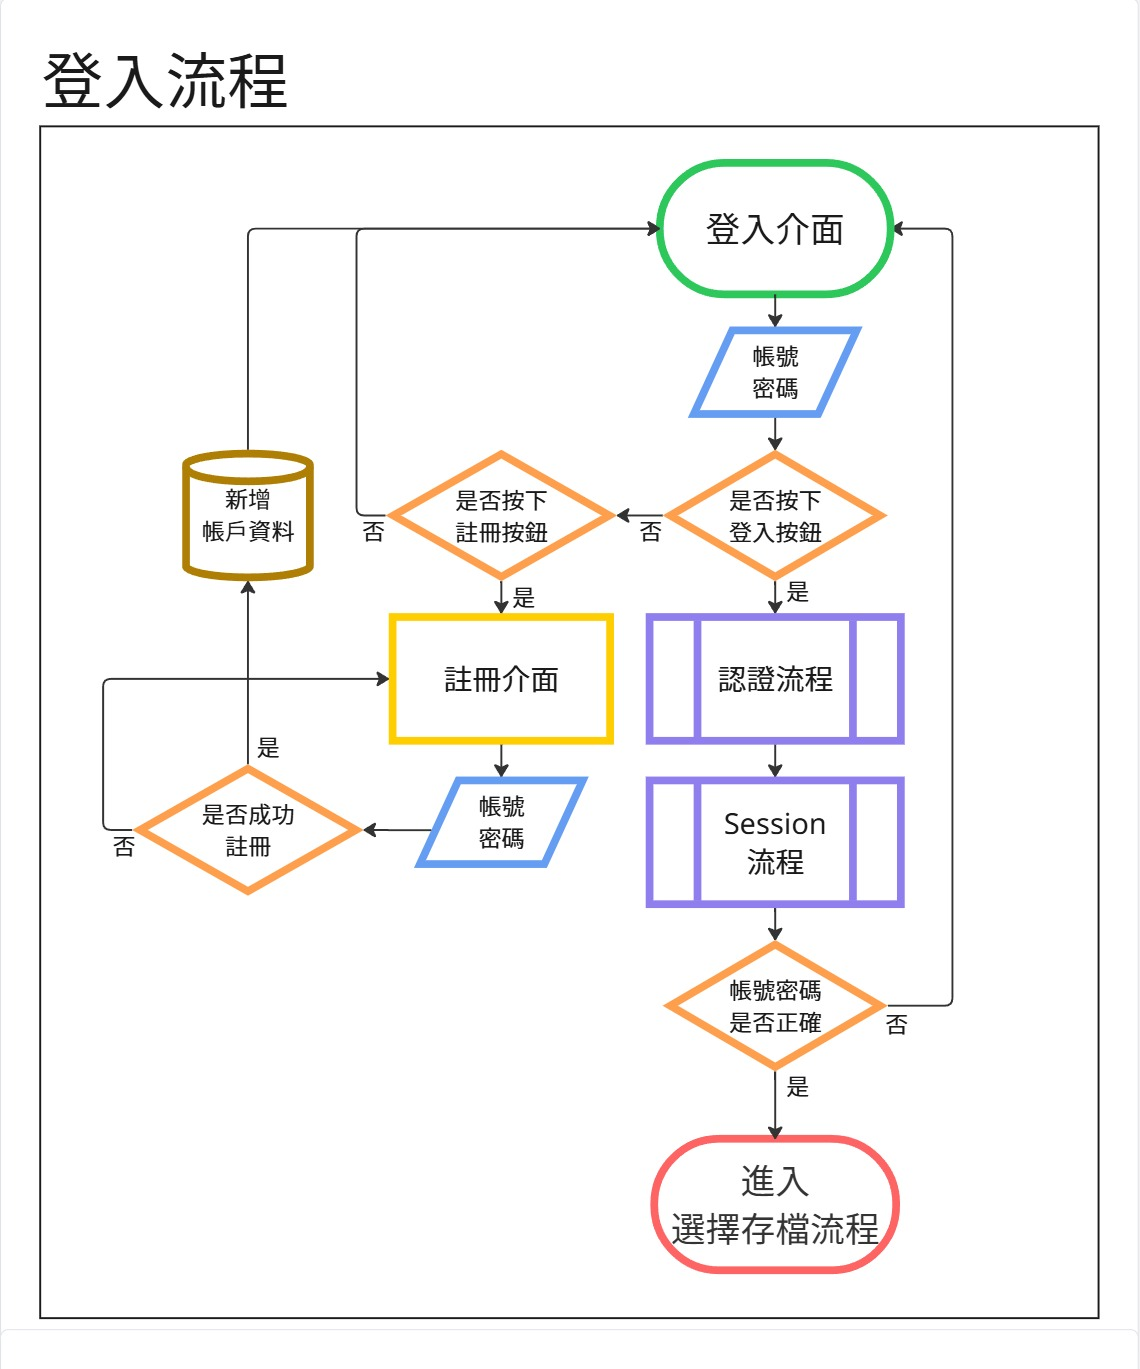
\includegraphics[width=\linewidth]{flowchart/1_login.jpg}
        %         \caption{登入與註冊流程圖}
        %         \label{fig:flow_login}
        %     \end{minipage}%
        %     \hfill % 自動填補兩張圖中間的空白，防止擠到下一行
        %     % 第二張圖 (佔據 48% 寬度)
        %     \begin{minipage}[t]{0.48\textwidth}
        %         \centering
        %         \includegraphics[width=\linewidth]{flowchart/2_savefile.jpg}
        %         \caption{選擇與建立存檔流程圖}
        %         \label{fig:flow_savefile}
        %     \end{minipage}
        % \end{figure}
        
        \begin{figure}[H]
            \centering
            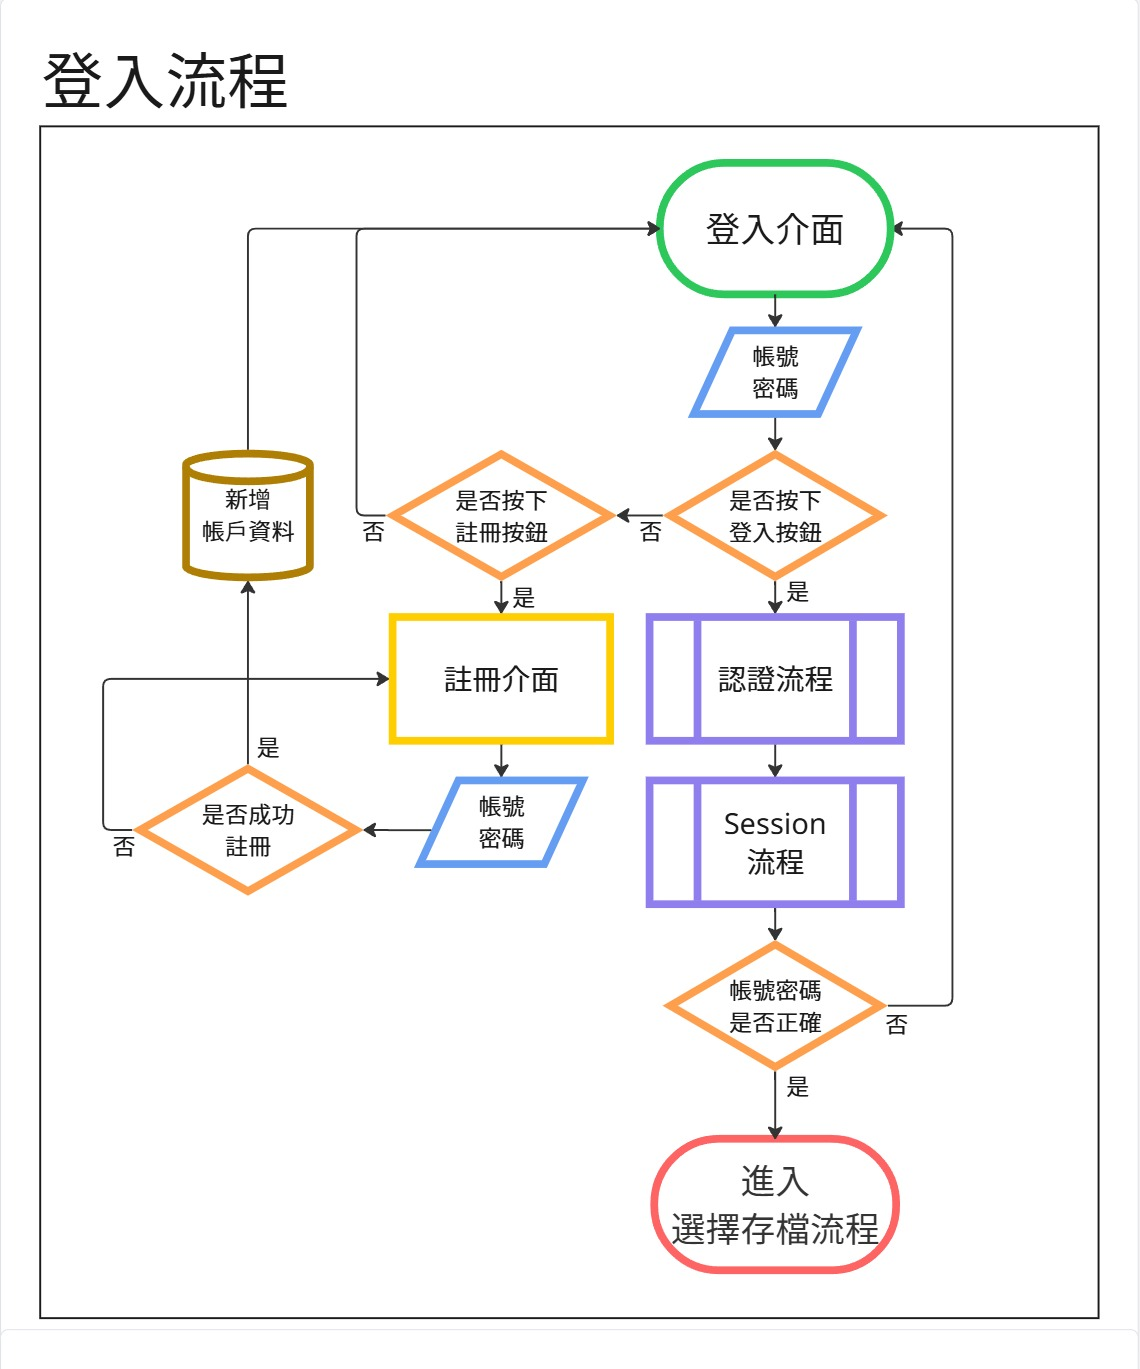
\includegraphics[width=0.5\textwidth]{flowchart/1_login.jpg}
            \caption{登入與註冊流程圖}
            \label{fig:flow_login}
        \end{figure}
        \begin{figure}[H]
            \centering
            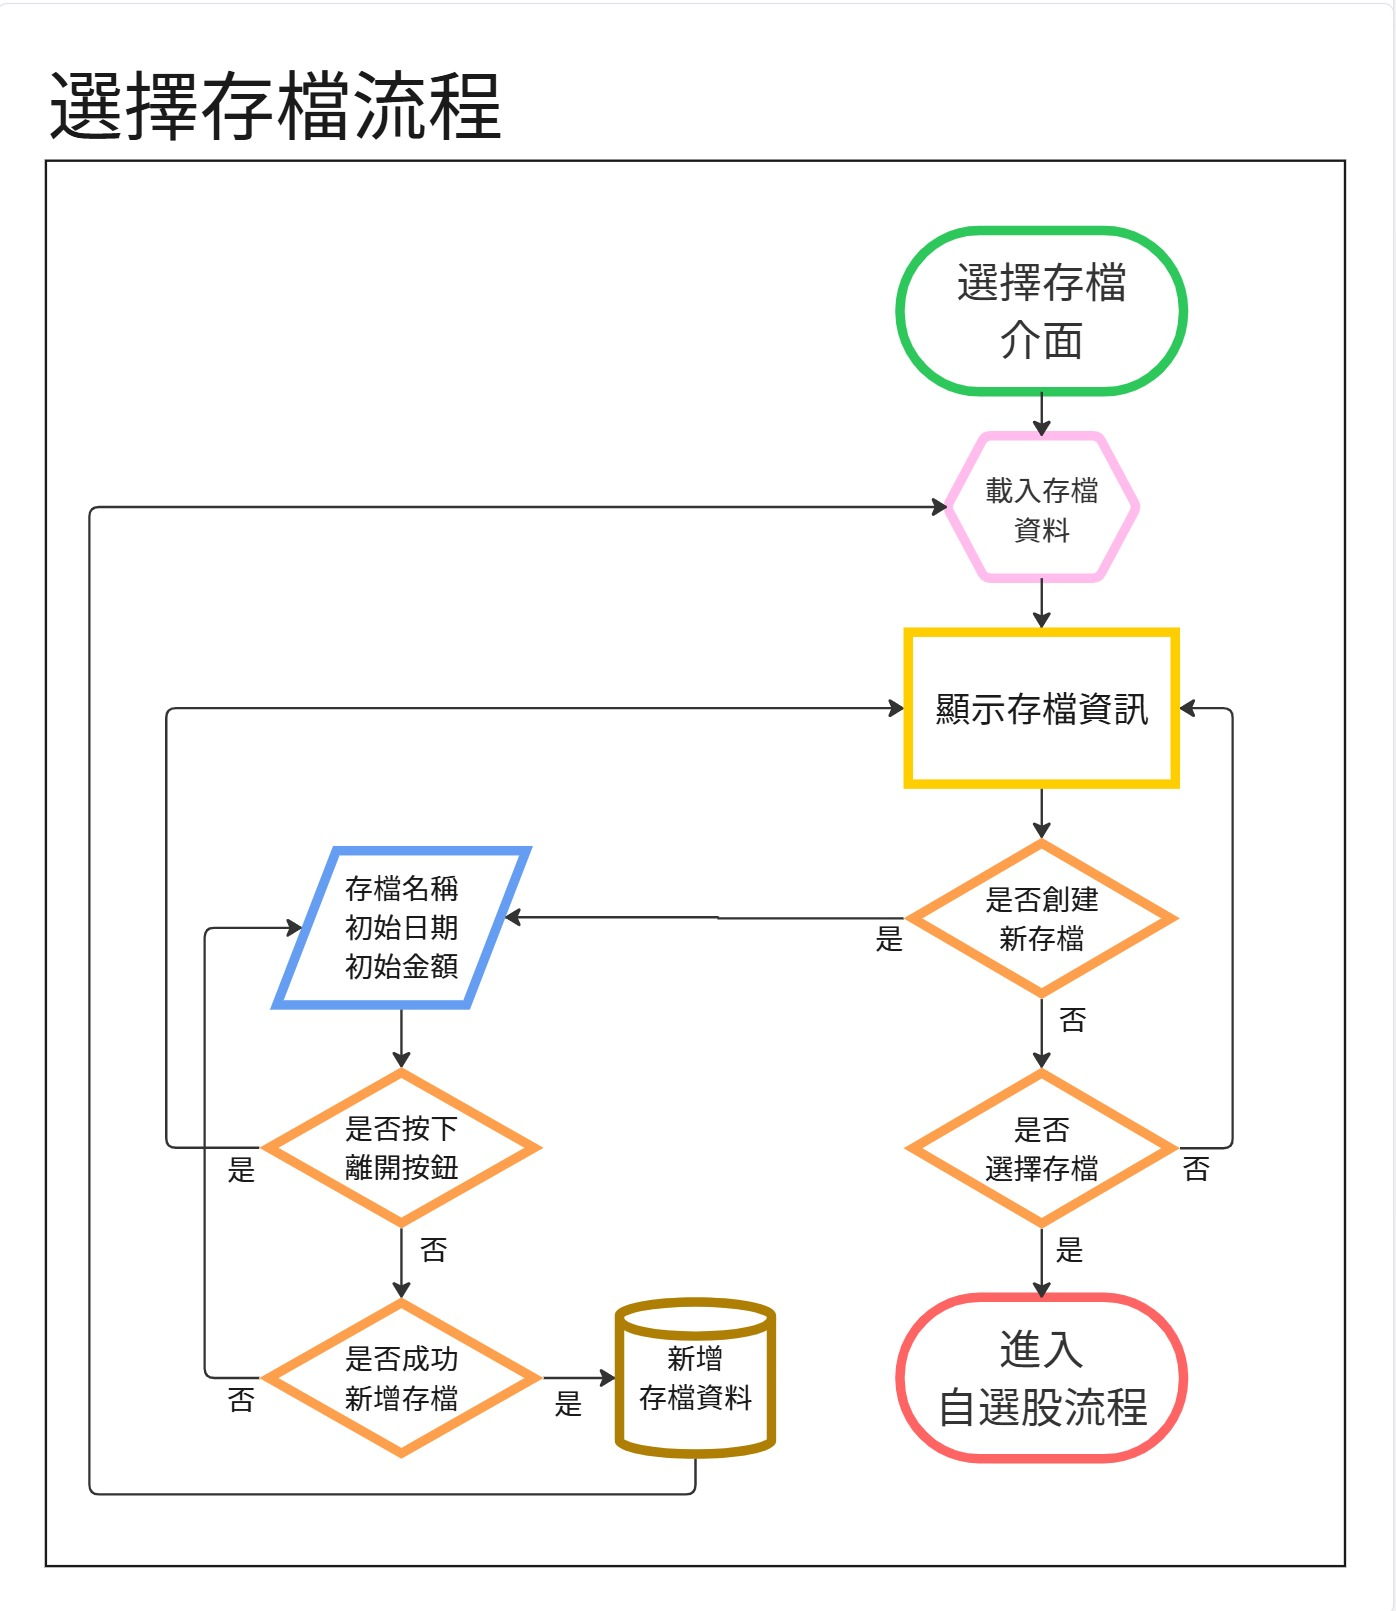
\includegraphics[width=0.5\textwidth]{flowchart/3_select_savefile.png}
            \caption{選擇與建立存檔流程圖}
            \label{fig:flow_select_savefile}
        \end{figure}

        \item \textbf{自選股主頁面流程 (Watchlist Hall Flow)} \\
        加載存檔後進入的主控制大廳（對應「自選」分頁）。頂端藍色狀態列即時顯示當前虛擬日期、時間階段、存款戶及交割戶餘額。頁面中央展示自選股清單（包含代碼、名稱、股價、漲跌與漲跌幅），並提供黃色按鈕以新增股票至清單；點擊綠色的時間推進按鈕，即可將交易階段向後推進並觸發撮合引擎。
        \begin{figure}[H]
            \centering
            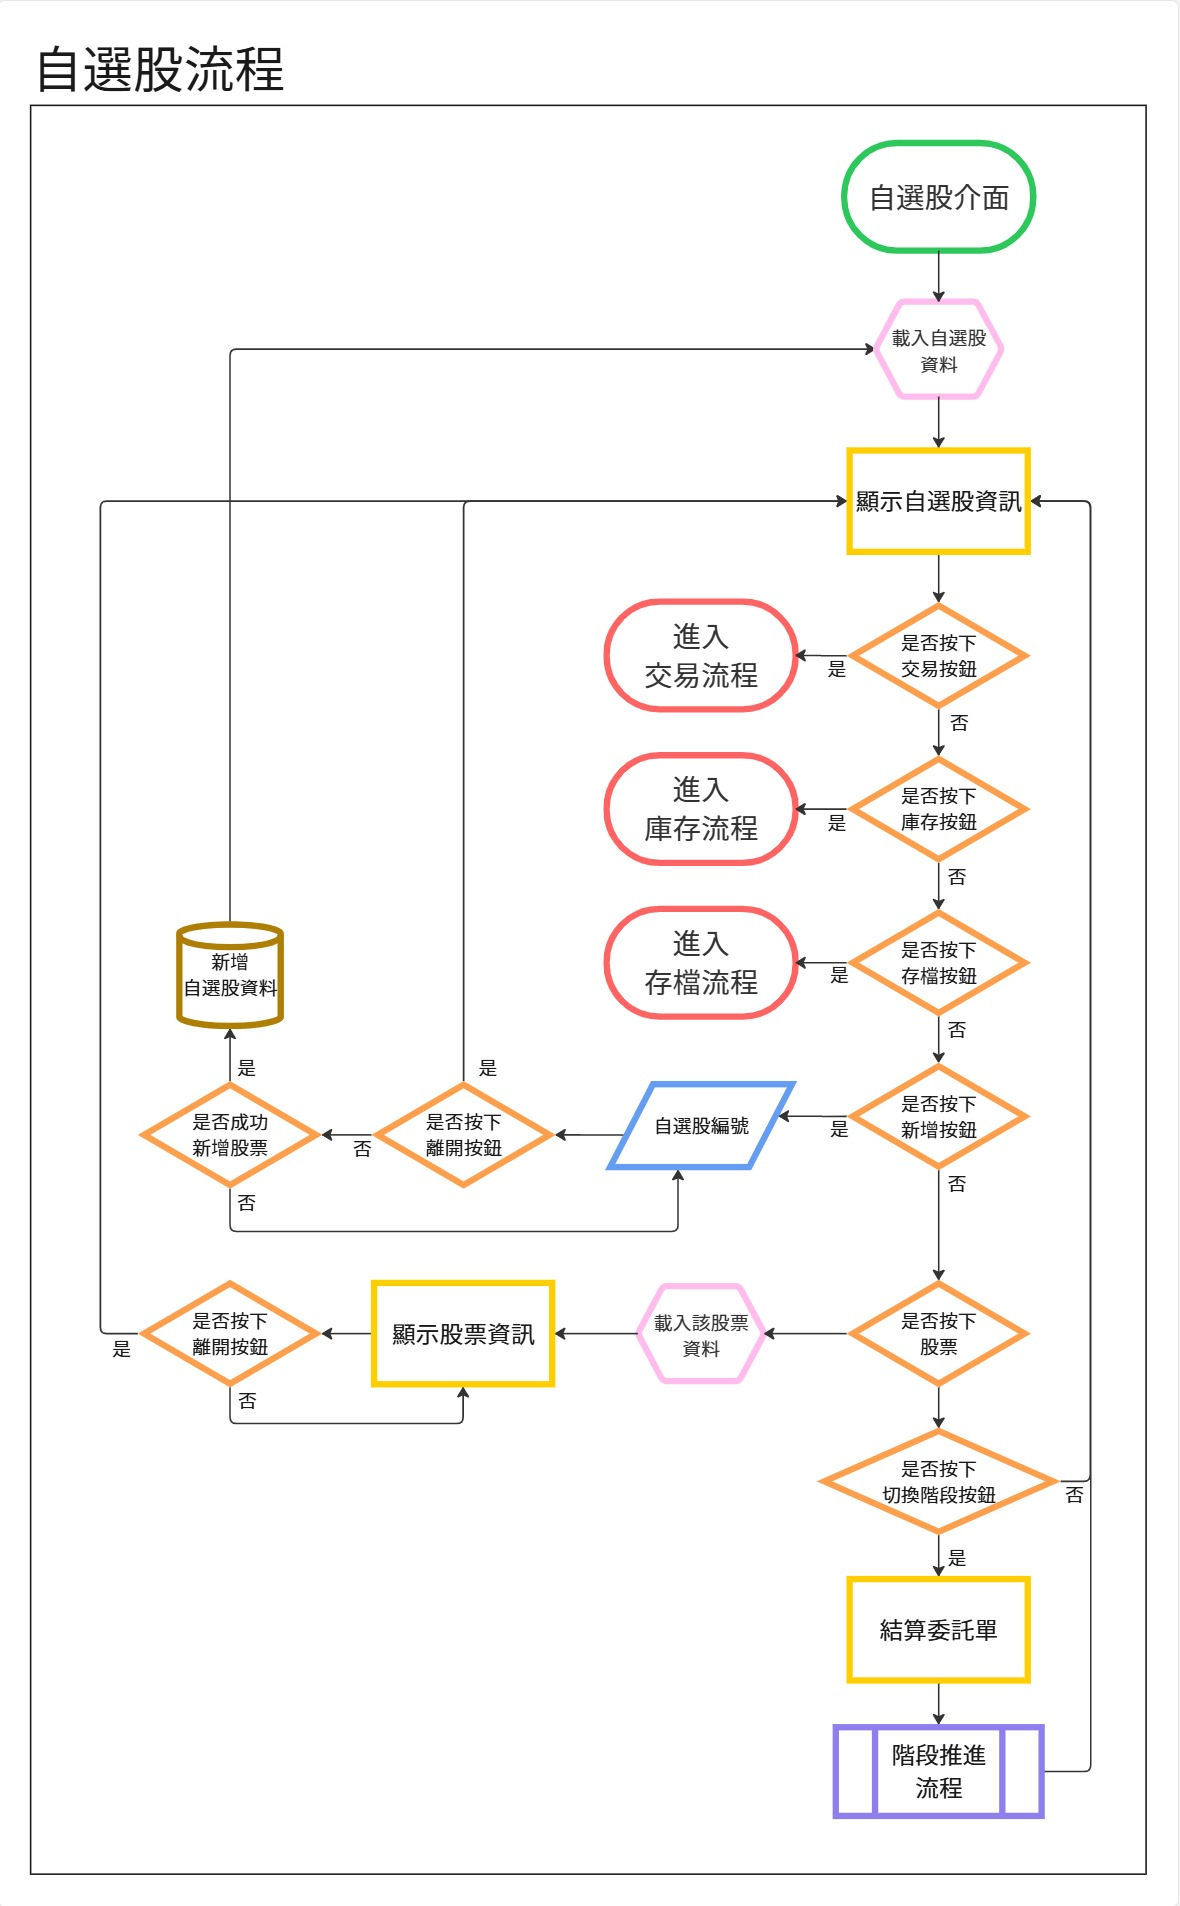
\includegraphics[width=0.65\textwidth]{flowchart/4_watchlist.png}
            \caption{自選股主頁面流程圖}
            \label{fig:flow_watchlist}
        \end{figure}

        \item \textbf{交易下單流程 (Trading Flow)} \\
        當玩家切換至「交易」分頁後進入。玩家可在此輸入股票代碼、委託價格與委託張數。系統提供直觀的切換開關（Switch）來選擇交易方向（買進/賣出）與委託類型（限價/市價）。送出前系統會自動驗證資金或庫存是否足夠，並將合法的委託單寫入資料庫等待交易撮合。
        \begin{figure}[H]
            \centering
            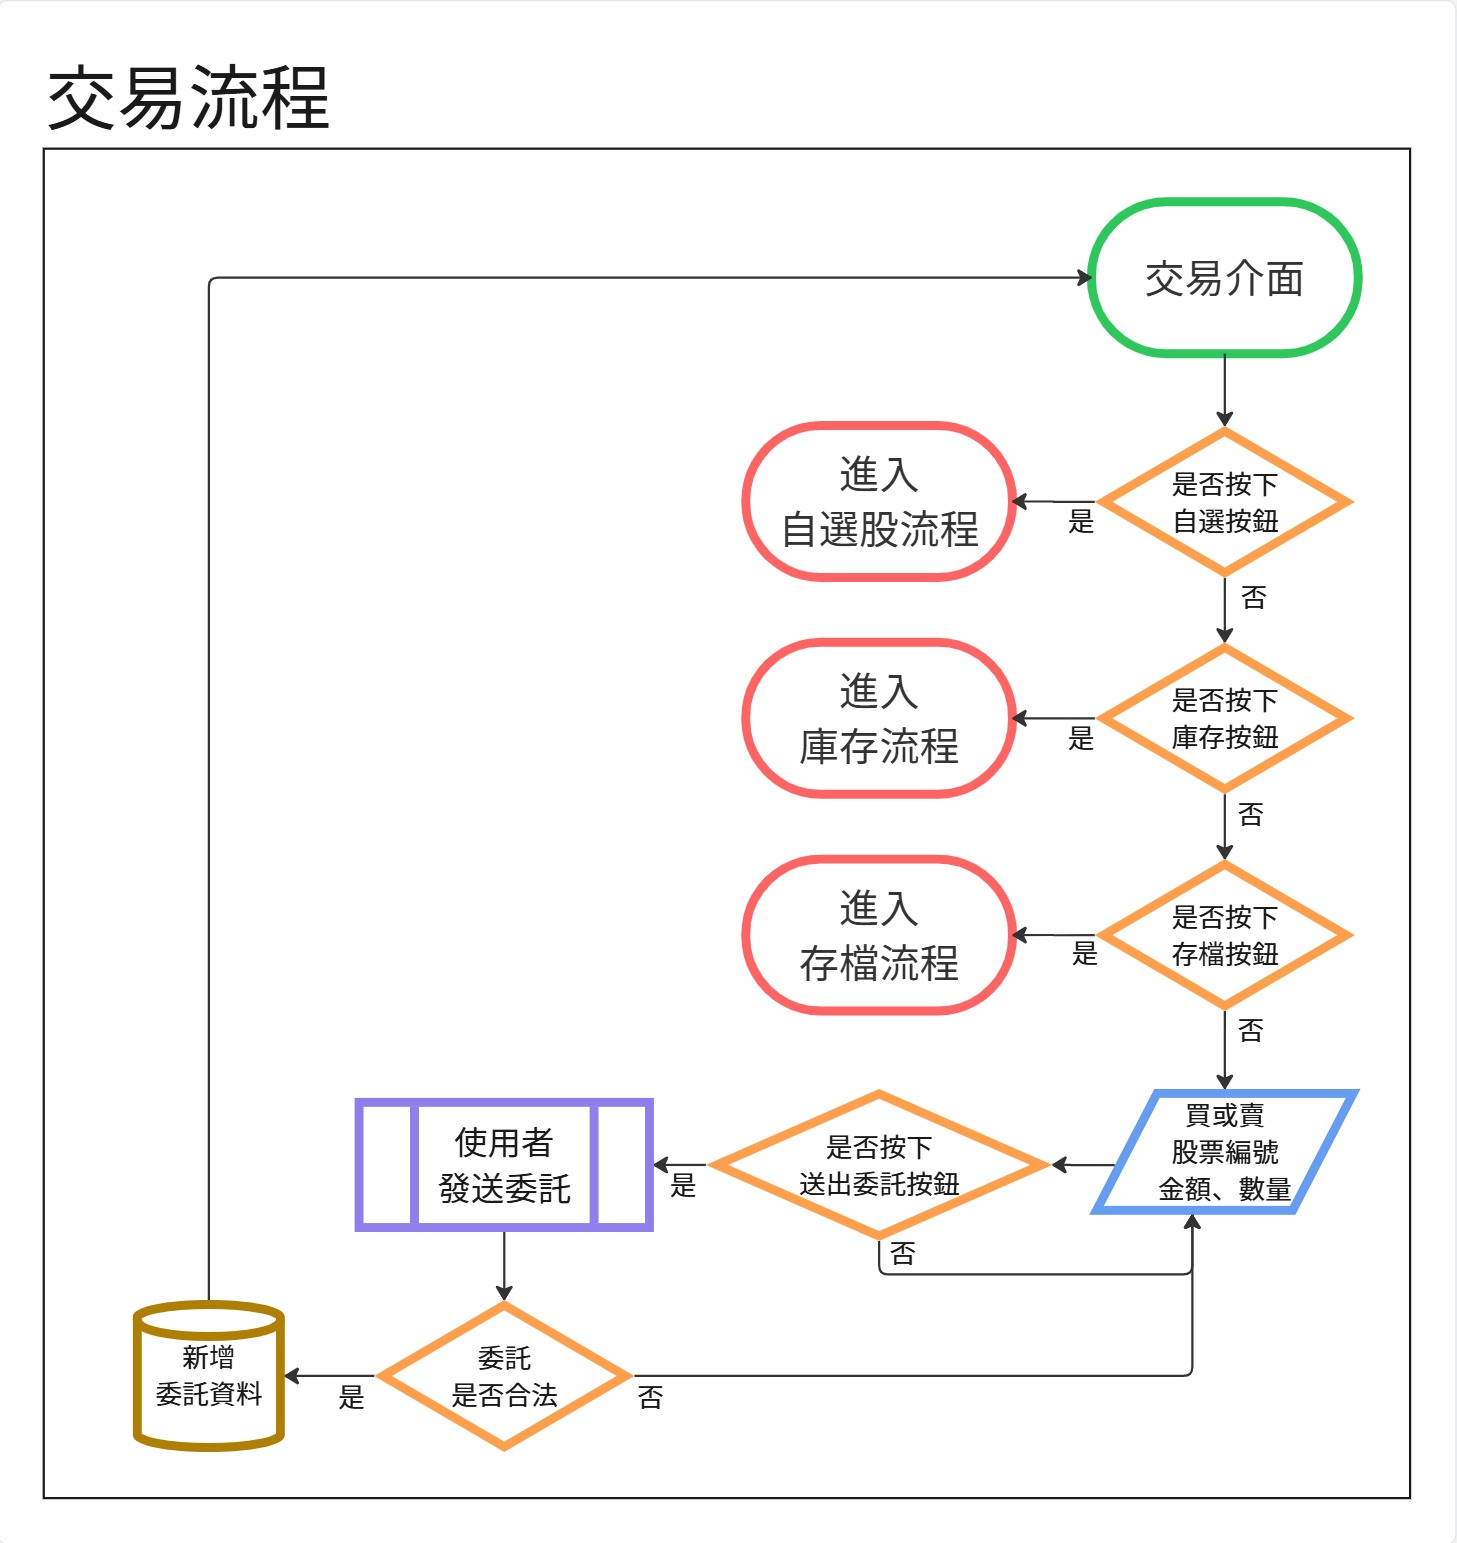
\includegraphics[width=0.8\textwidth]{flowchart/6_transact.png}
            \caption{交易下單流程圖}
            \label{fig:flow_transact}
        \end{figure}
        \newpage
        \item \textbf{資產庫存與轉帳流程 (Portfolio \& Bank Flow)} \\
        對應「庫存」分頁。上半部展示交割戶與存款戶的目前餘額，並提供雙向轉帳介面（輸入金額後點擊轉帳圖示即可即時互轉並寫入金流帳本）；下半部則顯示持股庫存清單，包含代碼、名稱、持股數量、損益、獲利率、現價與加權平均成本，方便玩家評估未實現損益。
        \begin{figure}[H]
            \centering
            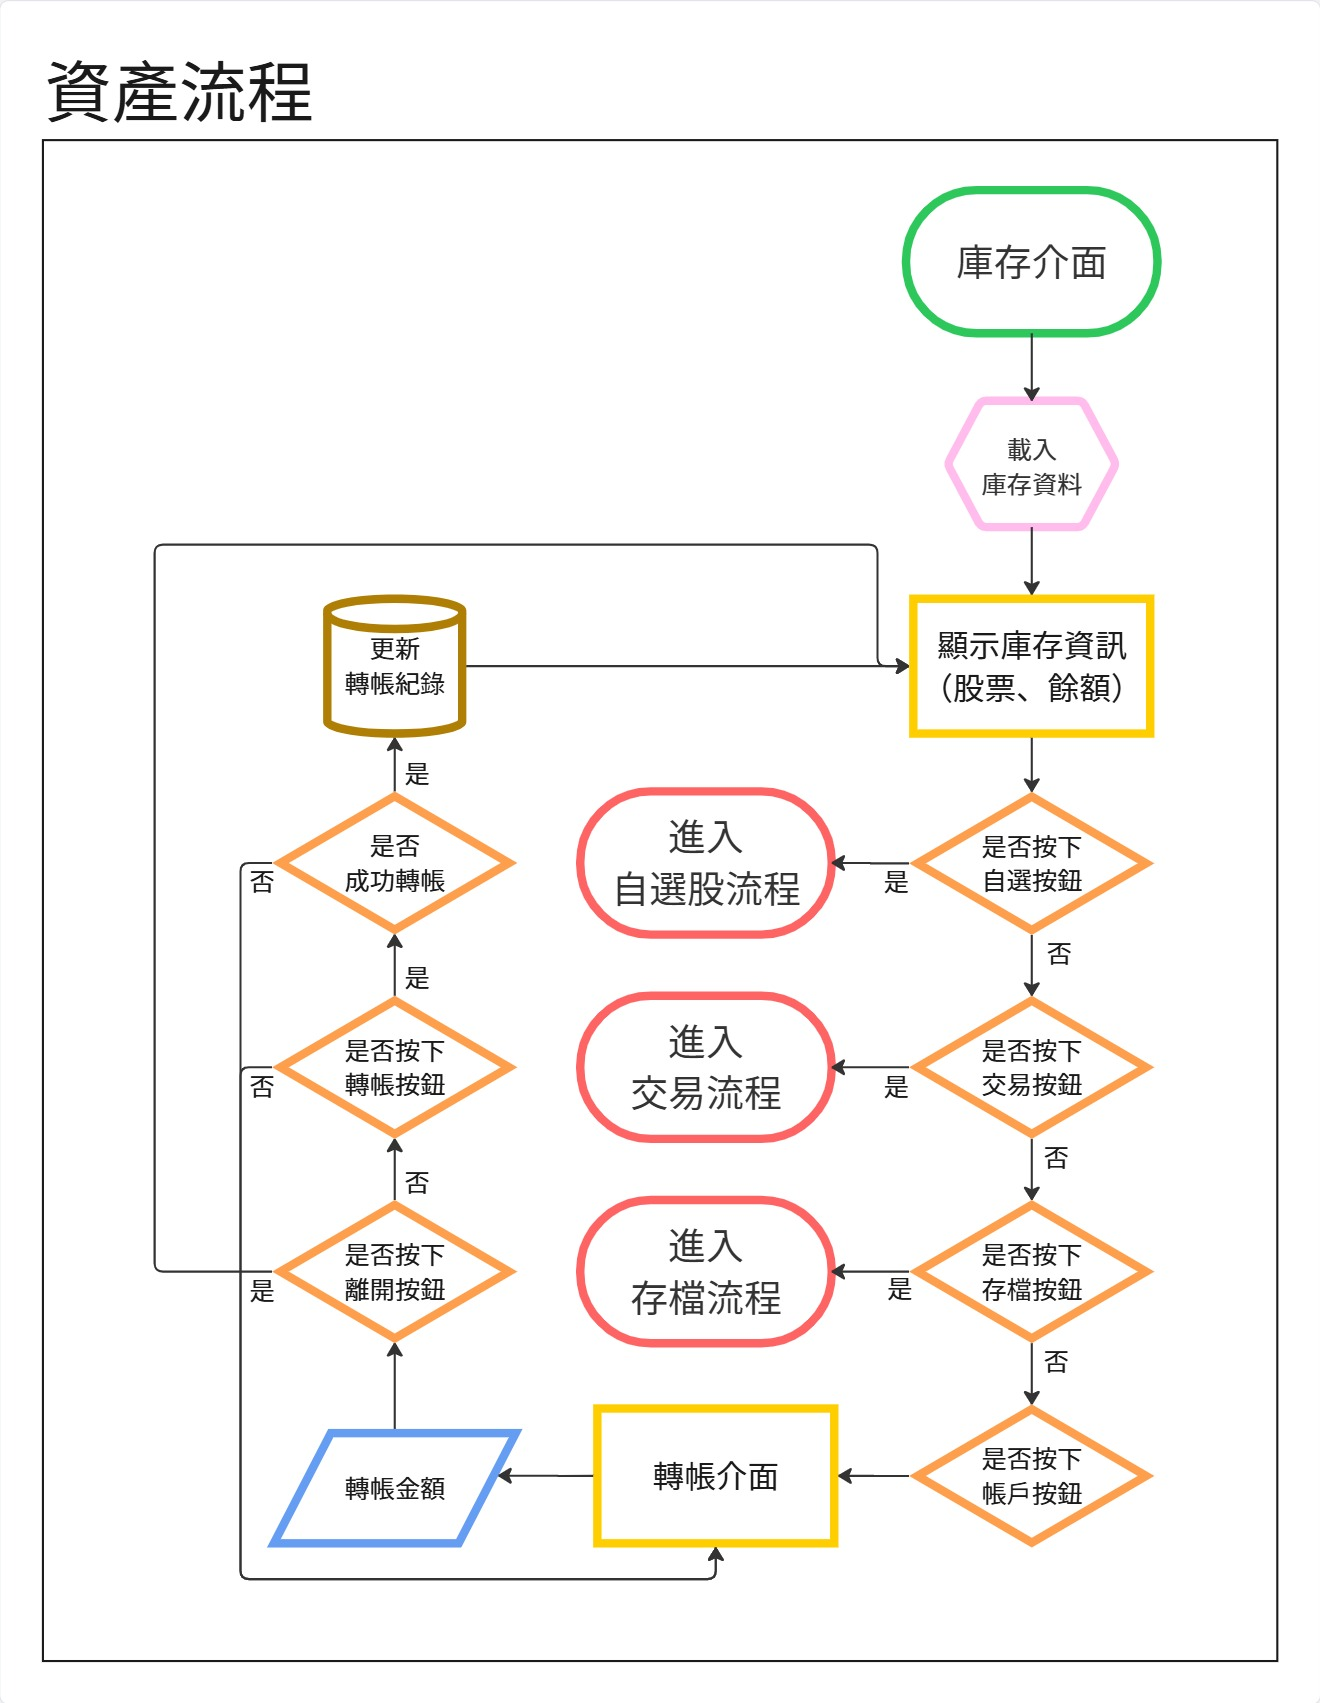
\includegraphics[width=0.8\textwidth]{flowchart/8_account.png}
            \caption{資產庫存與轉帳流程圖}
            \label{fig:flow_account}
        \end{figure}
        \newpage
        \item \textbf{紀錄選單 lobby 流程 (Record Menu Flow)} \\
        在「存檔」分頁中，玩家可查看當前存檔的整體績效與歷史數據。頁面右上方設有切換下拉式選單（Drop-down Menu），作為各項歷史紀錄的整合入口，玩家可在此選擇要檢視交易明細、帳戶轉帳紀錄或管理存檔。
        \begin{figure}[H]
            \centering
            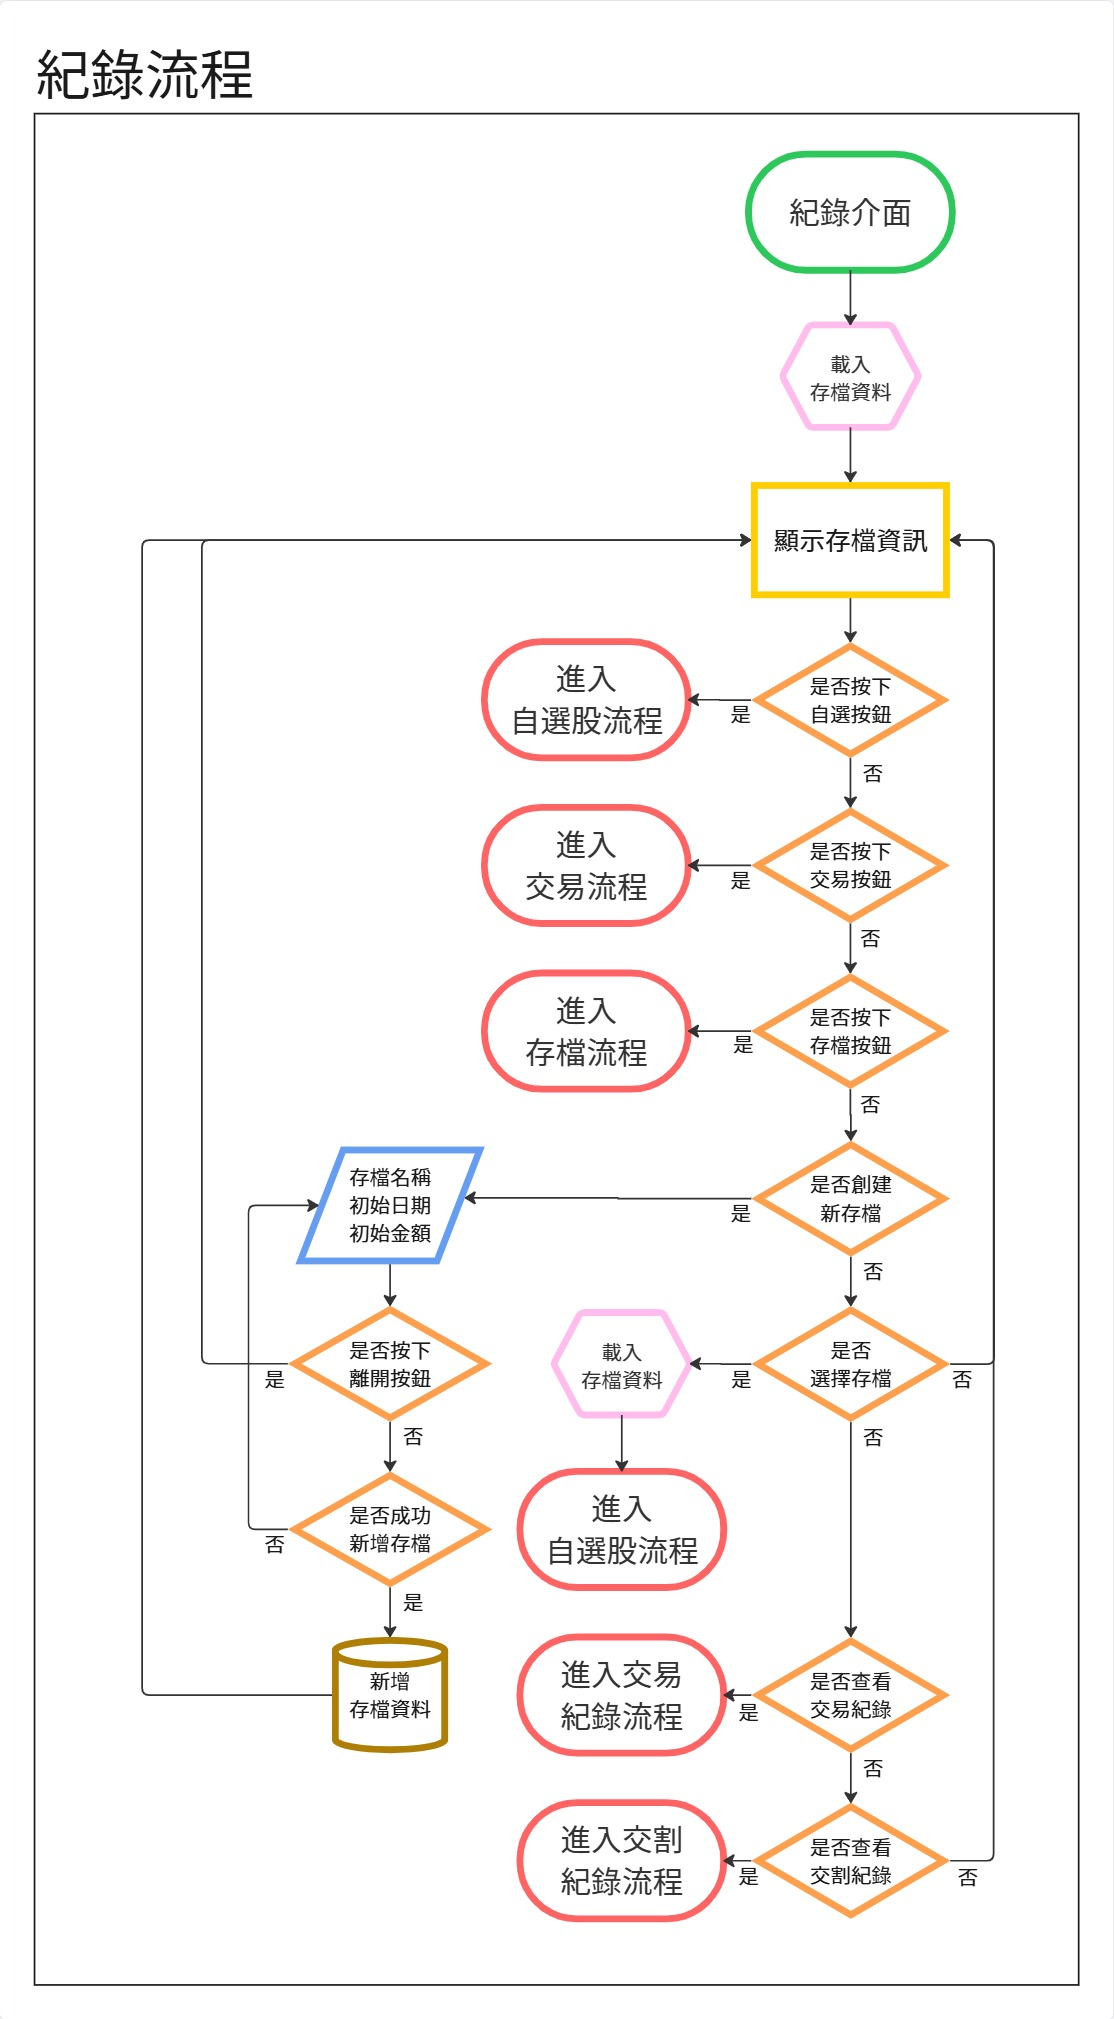
\includegraphics[width=0.62\textwidth]{flowchart/9_record_savefile.png}
            \caption{紀錄選單流程圖}
            \label{fig:flow_record_savefile}
        \end{figure}
        \newpage
        \item \textbf{交易與交割紀錄流程 (History Records Flow)} \\
        透過「存檔」分頁的下拉式選單，玩家可切換至「交易紀錄」或「轉帳紀錄」表格。「交易紀錄」詳細列出歷次成交的股票名稱、損益、報酬率、交易類別、成交股數與價格、出帳金額與投資成本；「轉帳紀錄」則列出交割戶與存款戶的資金異動明細，以利玩家進行績效評估與對帳。
        \begin{figure}[H]
            \centering
            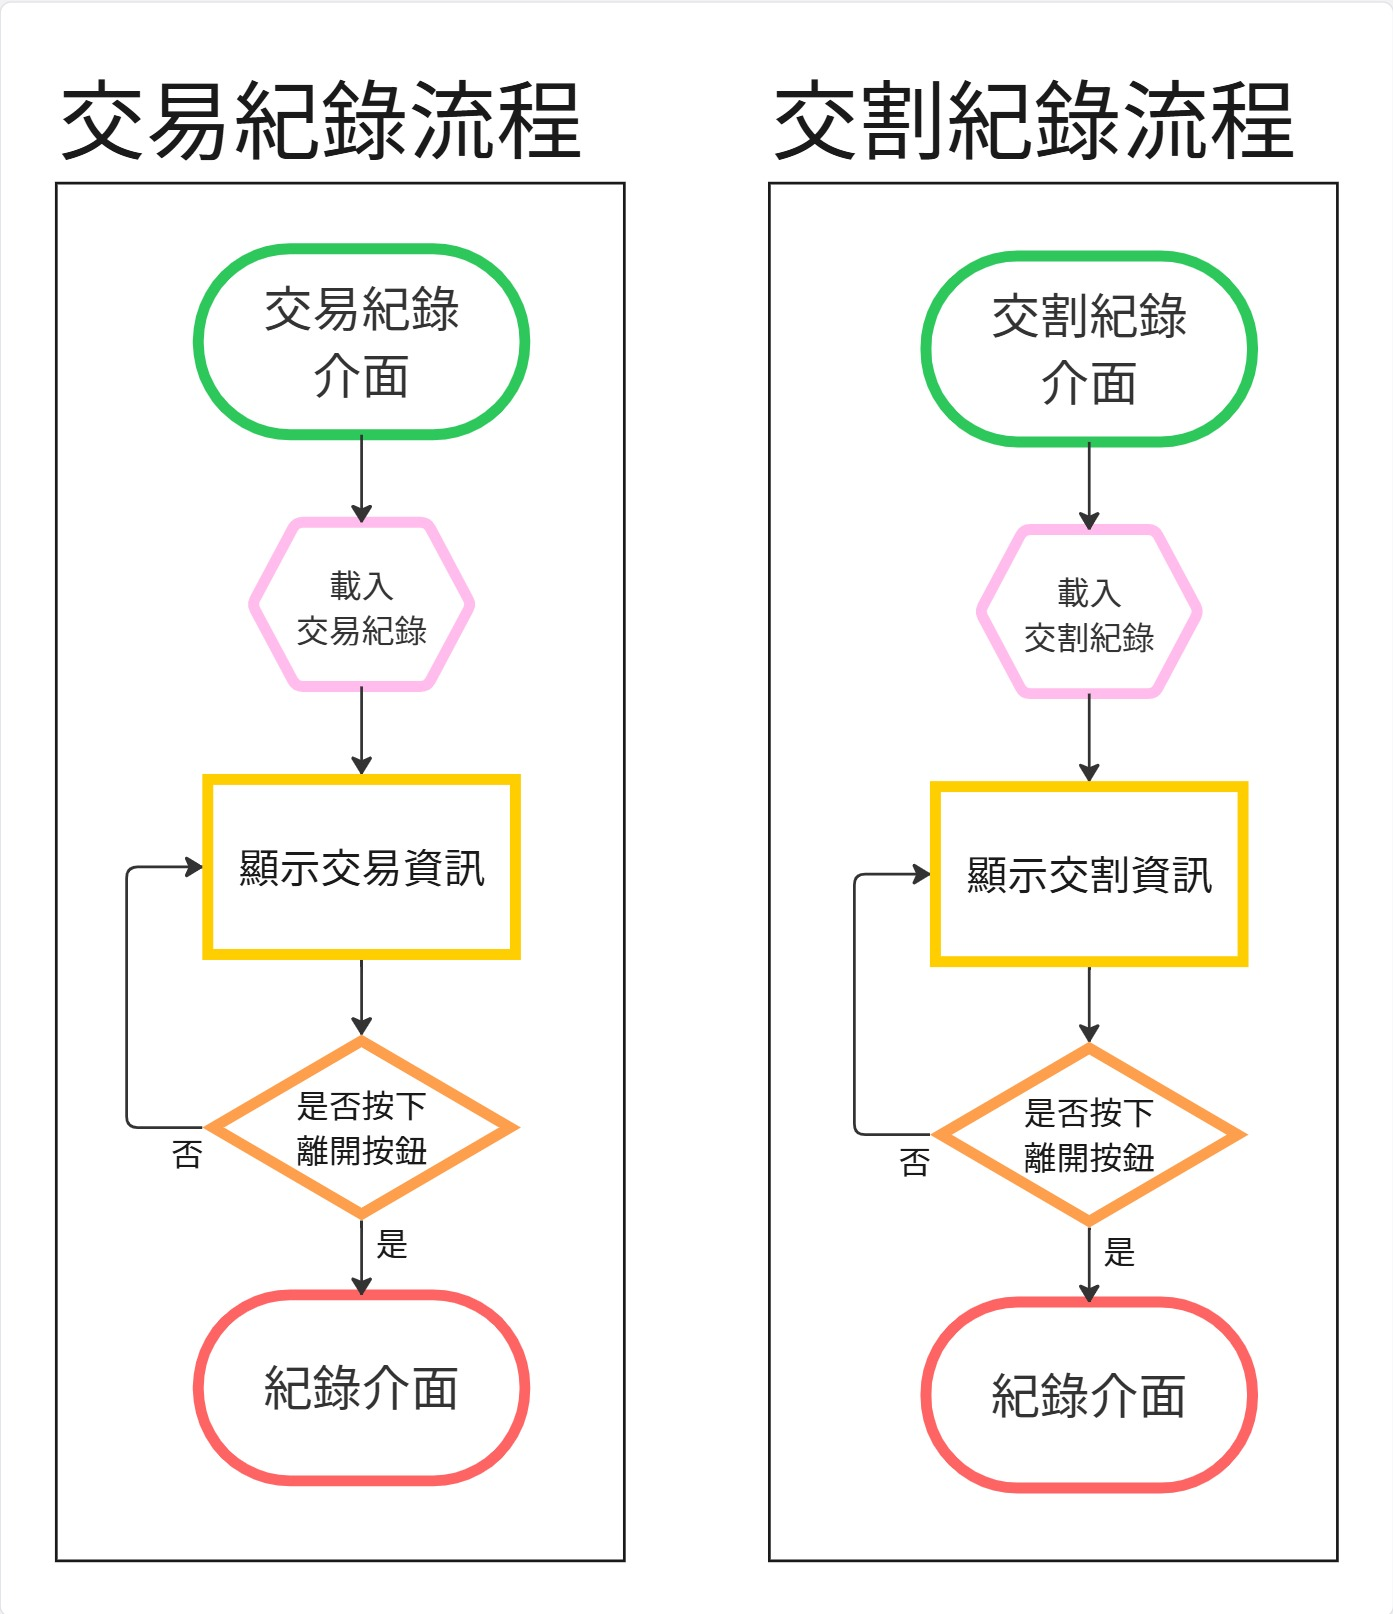
\includegraphics[width=0.85\textwidth]{flowchart/10_watch_transact.png}
            \caption{交易與交割紀錄流程圖}
            \label{fig:flow_watch_transact}
        \end{figure}
    \end{enumerate}

    \subsubsection{後端 API 與業務邏輯流程}
    本系統的後端 API 與核心業務邏輯流程，包括身分驗證與單一登入防呆、交易日與階段切換、以及委託單下單與撮合引擎結算。以下為其詳細運作邏輯：

    \begin{figure}[H]
        \centering
        \resizebox{0.95\textwidth}{!}{
            \begin{tikzpicture}[
                auto,
                block/.style={rectangle, draw, thick, fill=blue!5, text width=4cm, align=center, minimum height=0.8cm, font=\sffamily},
                decision/.style={diamond, draw, thick, fill=yellow!10, text width=2.5cm, align=center, inner sep=1pt, font=\sffamily},
                process/.style={rectangle, draw, thick, rounded corners, fill=green!5, text width=4cm, align=center, minimum height=0.8cm, font=\sffamily},
                line/.style={draw, thick, -{Stealth[length=3mm]}}
            ]
                % Subgraph REG: Register
                \node[block] (reg1) {送出帳號與密碼 \\ \texttt{POST /auth/register}};
                \node[decision, below=0.8cm of reg1] (reg2) {帳號已存在？};
                \node[process, right=1.2cm of reg2] (reg3) {回傳 409 \\ 帳號已存在};
                \node[block, below=0.8cm of reg2] (reg4) {使用 Bcrypt \\ 進行密碼雜湊};
                \node[block, below=0.8cm of reg4] (reg5) {寫入 \texttt{users} 表 \\ (\texttt{session\_id} 設為 \texttt{NULL})};
                \node[process, below=0.8cm of reg5] (reg6) {回傳 201 \\ 註冊成功};
                
                \path[line] (reg1) -- (reg2);
                \path[line] (reg2) -- node [above] {是} (reg3);
                \path[line] (reg2) -- node [left] {否} (reg4);
                \path[line] (reg4) -- (reg5);
                \path[line] (reg5) -- (reg6);
                
                % Subgraph LOGIN: Login
                \node[block, right=6.5cm of reg1] (log1) {送出帳號與密碼 \\ \texttt{POST /auth/login}};
                \node[decision, below=0.8cm of log1] (log2) {帳號存在？};
                \node[process, right=1.2cm of log2] (log3) {回傳 401 \\ 帳號或密碼錯誤};
                \node[decision, below=0.8cm of log2] (log4) {Bcrypt \\ 密碼驗證？};
                \node[block, below=0.8cm of log4] (log5) {生成全新安全憑證 \\ \texttt{session\_id}};
                \node[block, below=0.8cm of log5] (log6) {更新 \texttt{session\_id} \\ (迫使舊登入失效)};
                \node[process, below=0.8cm of log6] (log7) {回傳 200 \\ 登入與憑證成功};
                
                \path[line] (log1) -- (log2);
                \path[line] (log2) -- node [above] {否} (log3);
                \path[line] (log2) -- node [left] {是} (log4);
                \path[line] (log4) -- node [left] {是} (log5);
                \path[line] (log4.east) -- node [above right] {否} ++(1.2,0) -| (log3.south);
                \path[line] (log5) -- (log6);
                \path[line] (log6) -- (log7);
            \end{tikzpicture}
        }
        \caption{後端身分驗證（註冊與登入）流程圖}
        \label{fig:flow_auth}
    \end{figure}

    \begin{figure}[H]
        \centering
        \resizebox{0.95\textwidth}{!}{
            \begin{tikzpicture}[
                auto,
                block/.style={rectangle, draw, thick, fill=blue!5, text width=4cm, align=center, minimum height=0.8cm, font=\sffamily},
                decision/.style={diamond, draw, thick, fill=yellow!10, text width=2.5cm, align=center, inner sep=1pt, font=\sffamily},
                process/.style={rectangle, draw, thick, rounded corners, fill=green!5, text width=4cm, align=center, minimum height=0.8cm, font=\sffamily},
                line/.style={draw, thick, -{Stealth[length=3mm]}}
            ]
                % Middleware Validation
                \node[block] (mid1) {用戶請求受保護路由 \\ 攜帶 \texttt{X-Session-Id}};
                \node[decision, below=0.8cm of mid1] (mid2) {標頭是否存在？};
                \node[process, right=1.2cm of mid2] (mid3) {回傳 422 \\ 缺少驗證標頭};
                \node[decision, below=0.8cm of mid2] (mid4) {\texttt{session\_id} \\ 存在且對應有效？};
                \node[process, right=1.2cm of mid4] (mid5) {回傳 401 \\ 未授權登入};
                \node[process, below=0.8cm of mid4] (mid6) {注入 \texttt{current\_user} \\ 進入後續路由邏輯};
                
                \path[line] (mid1) -- (mid2);
                \path[line] (mid2) -- node [above] {否} (mid3);
                \path[line] (mid2) -- node [left] {是} (mid4);
                \path[line] (mid4) -- node [above] {否} (mid5);
                \path[line] (mid4) -- node [left] {是} (mid6);

                % Logout
                \node[block, right=6.5cm of mid1] (out1) {已驗證使用者 \\ \texttt{POST /auth/logout}};
                \node[process, below=1.2cm of out1] (out2) {更新 \texttt{session\_id} 為 \texttt{NULL} \\ 回傳 204 成功};
                \path[line] (out1) -- (out2);
            \end{tikzpicture}
        }
        \caption{受保護 API 請求驗證與登出流程圖}
        \label{fig:flow_middleware}
    \end{figure}

    \begin{figure}[H]
        \centering
        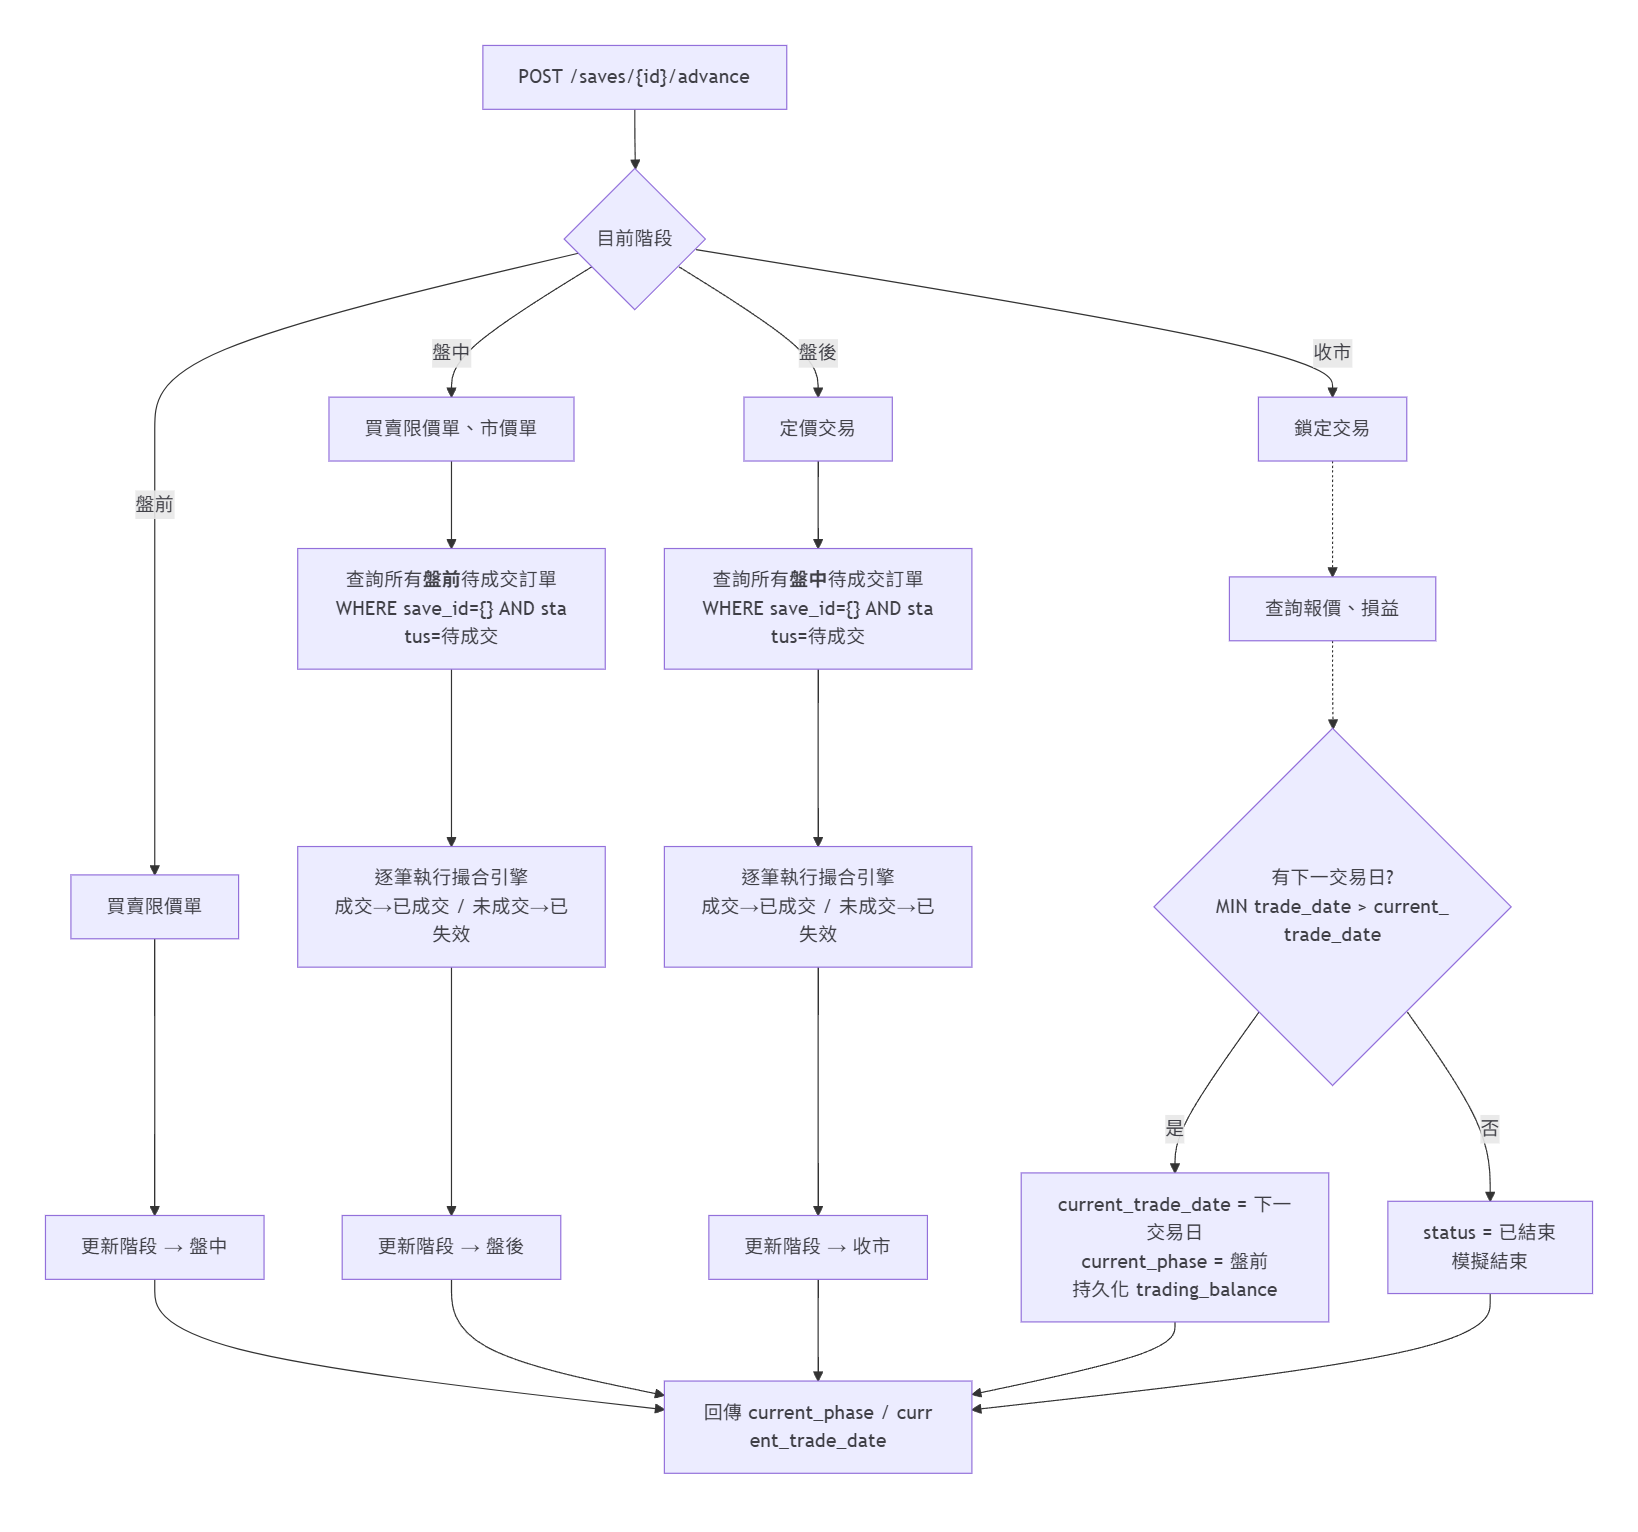
\includegraphics[width=0.95\textwidth]{flowchart/5_phase.png}
        \caption{階段推進邏輯圖}
        \label{fig:flow_phase}
    \end{figure}

    \begin{figure}[H]
        \centering
        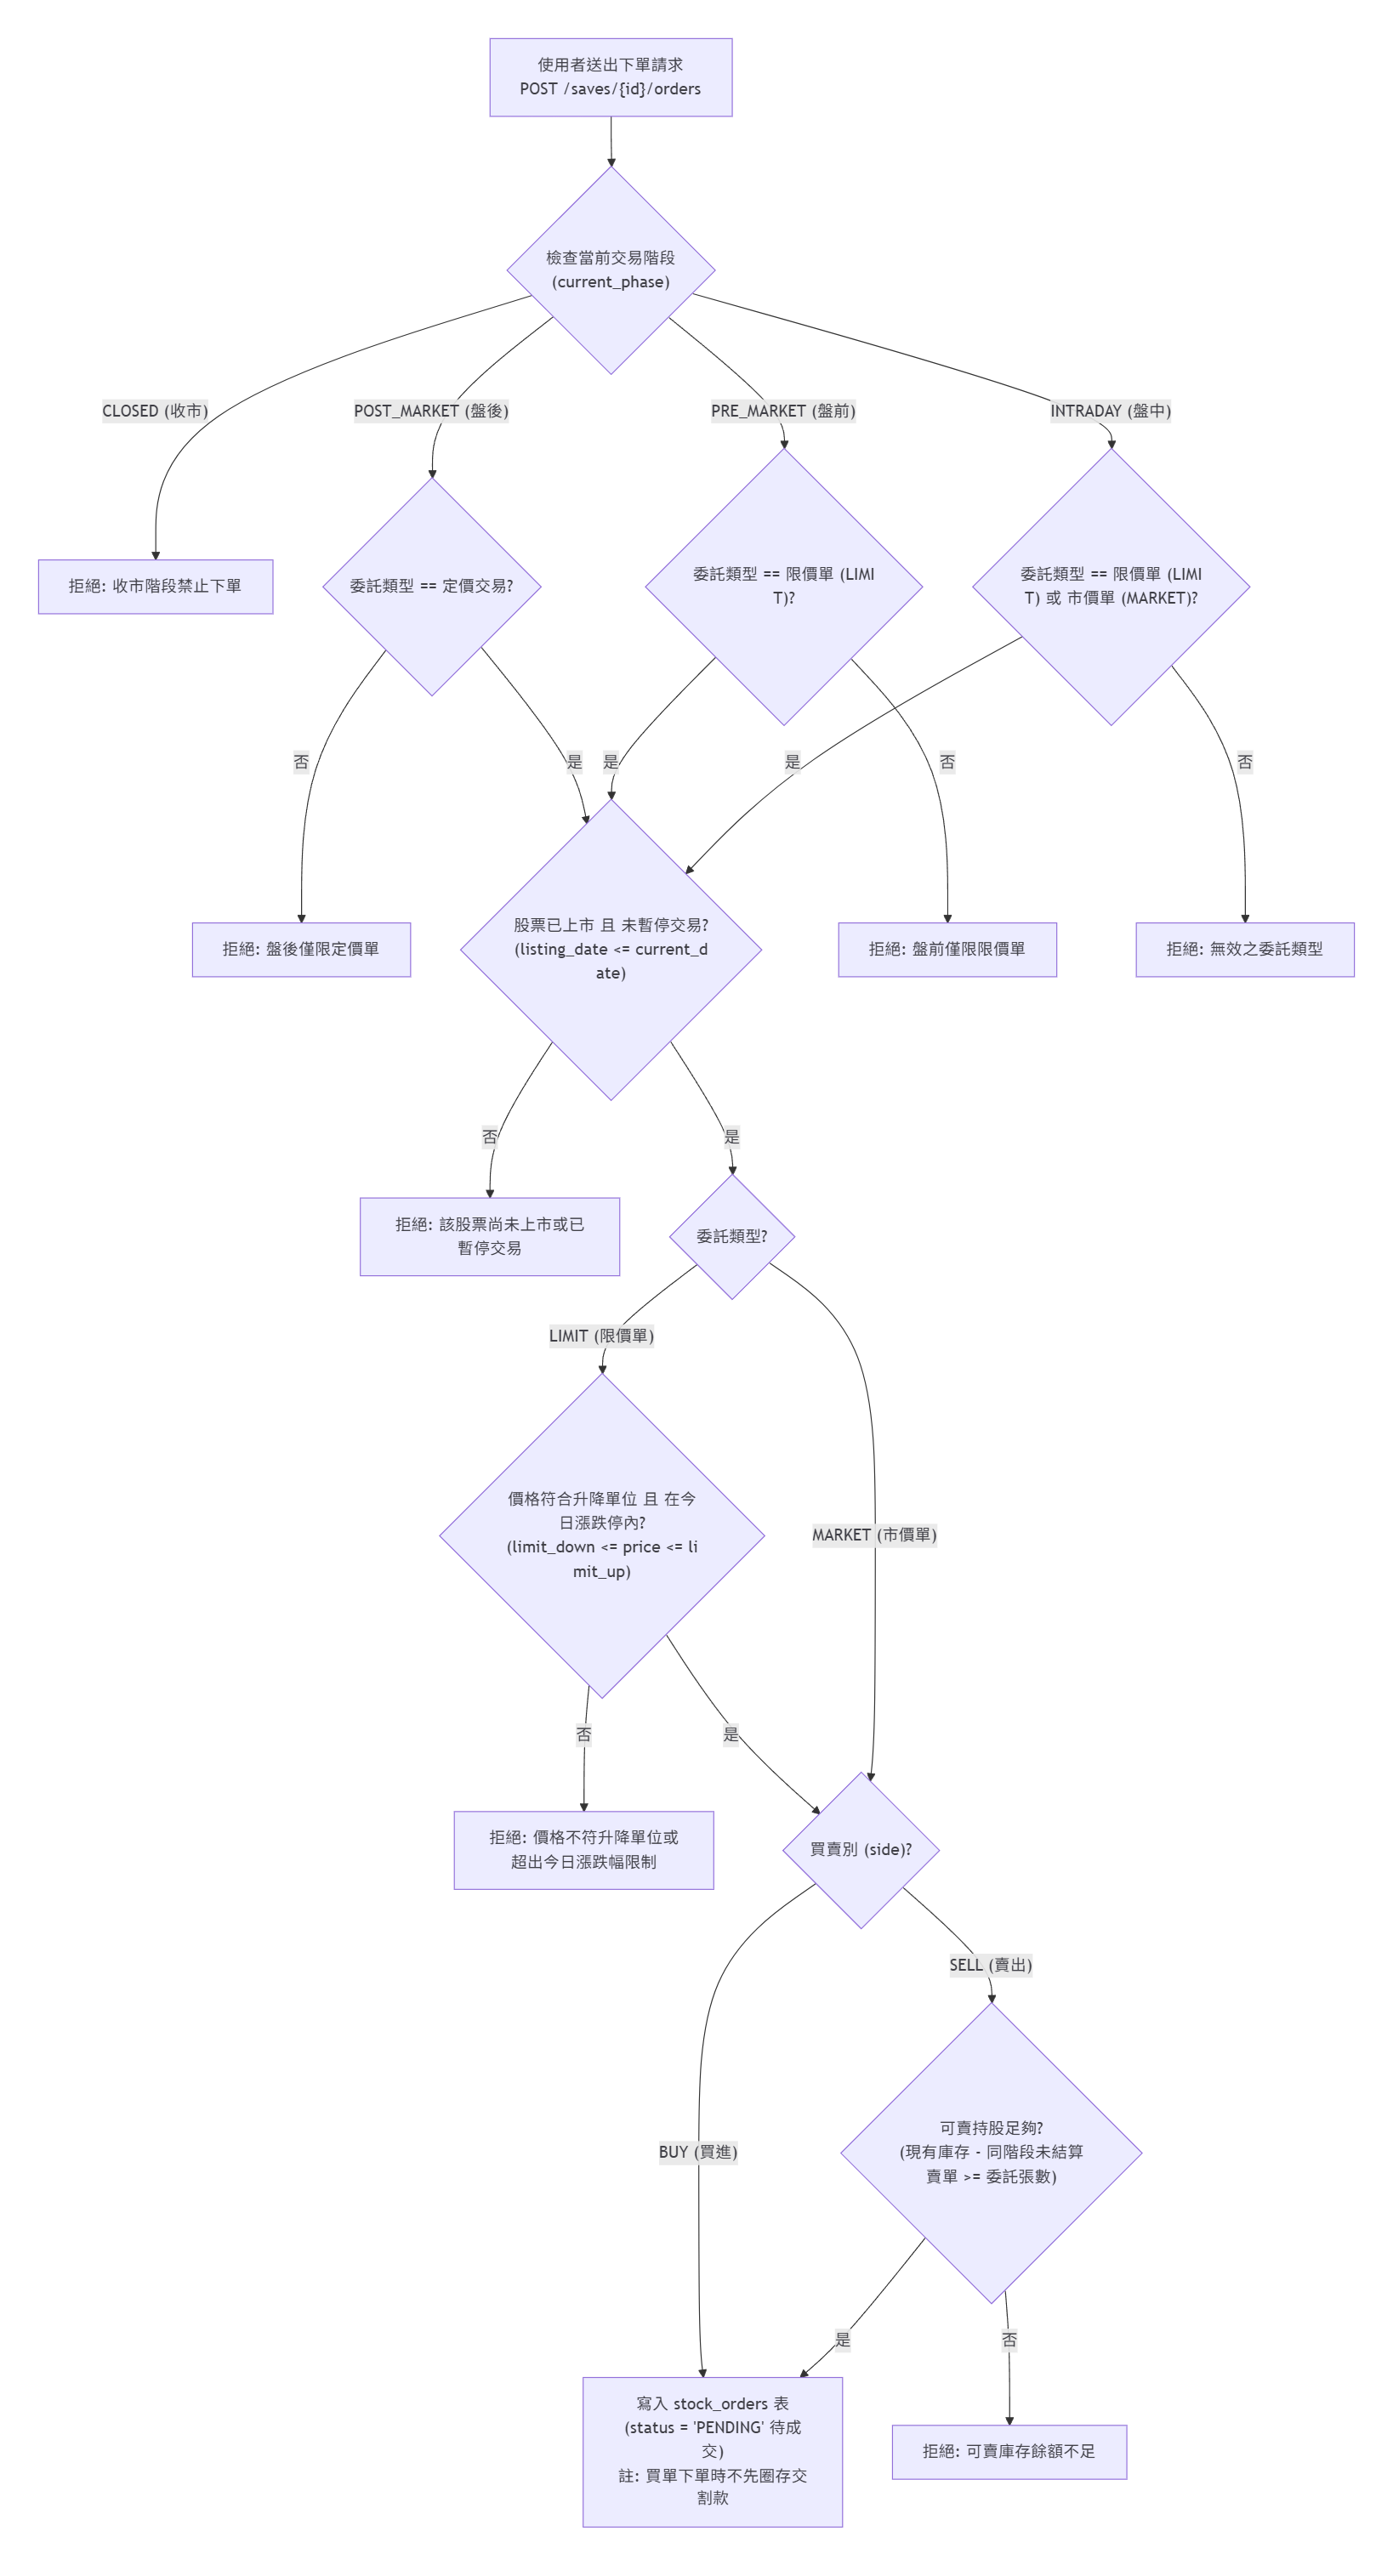
\includegraphics[width=0.75\textwidth]{flowchart/7_1_order.png}
        \caption{委託單流程圖}
    \end{figure}

    \begin{figure}[H]
        \centering
        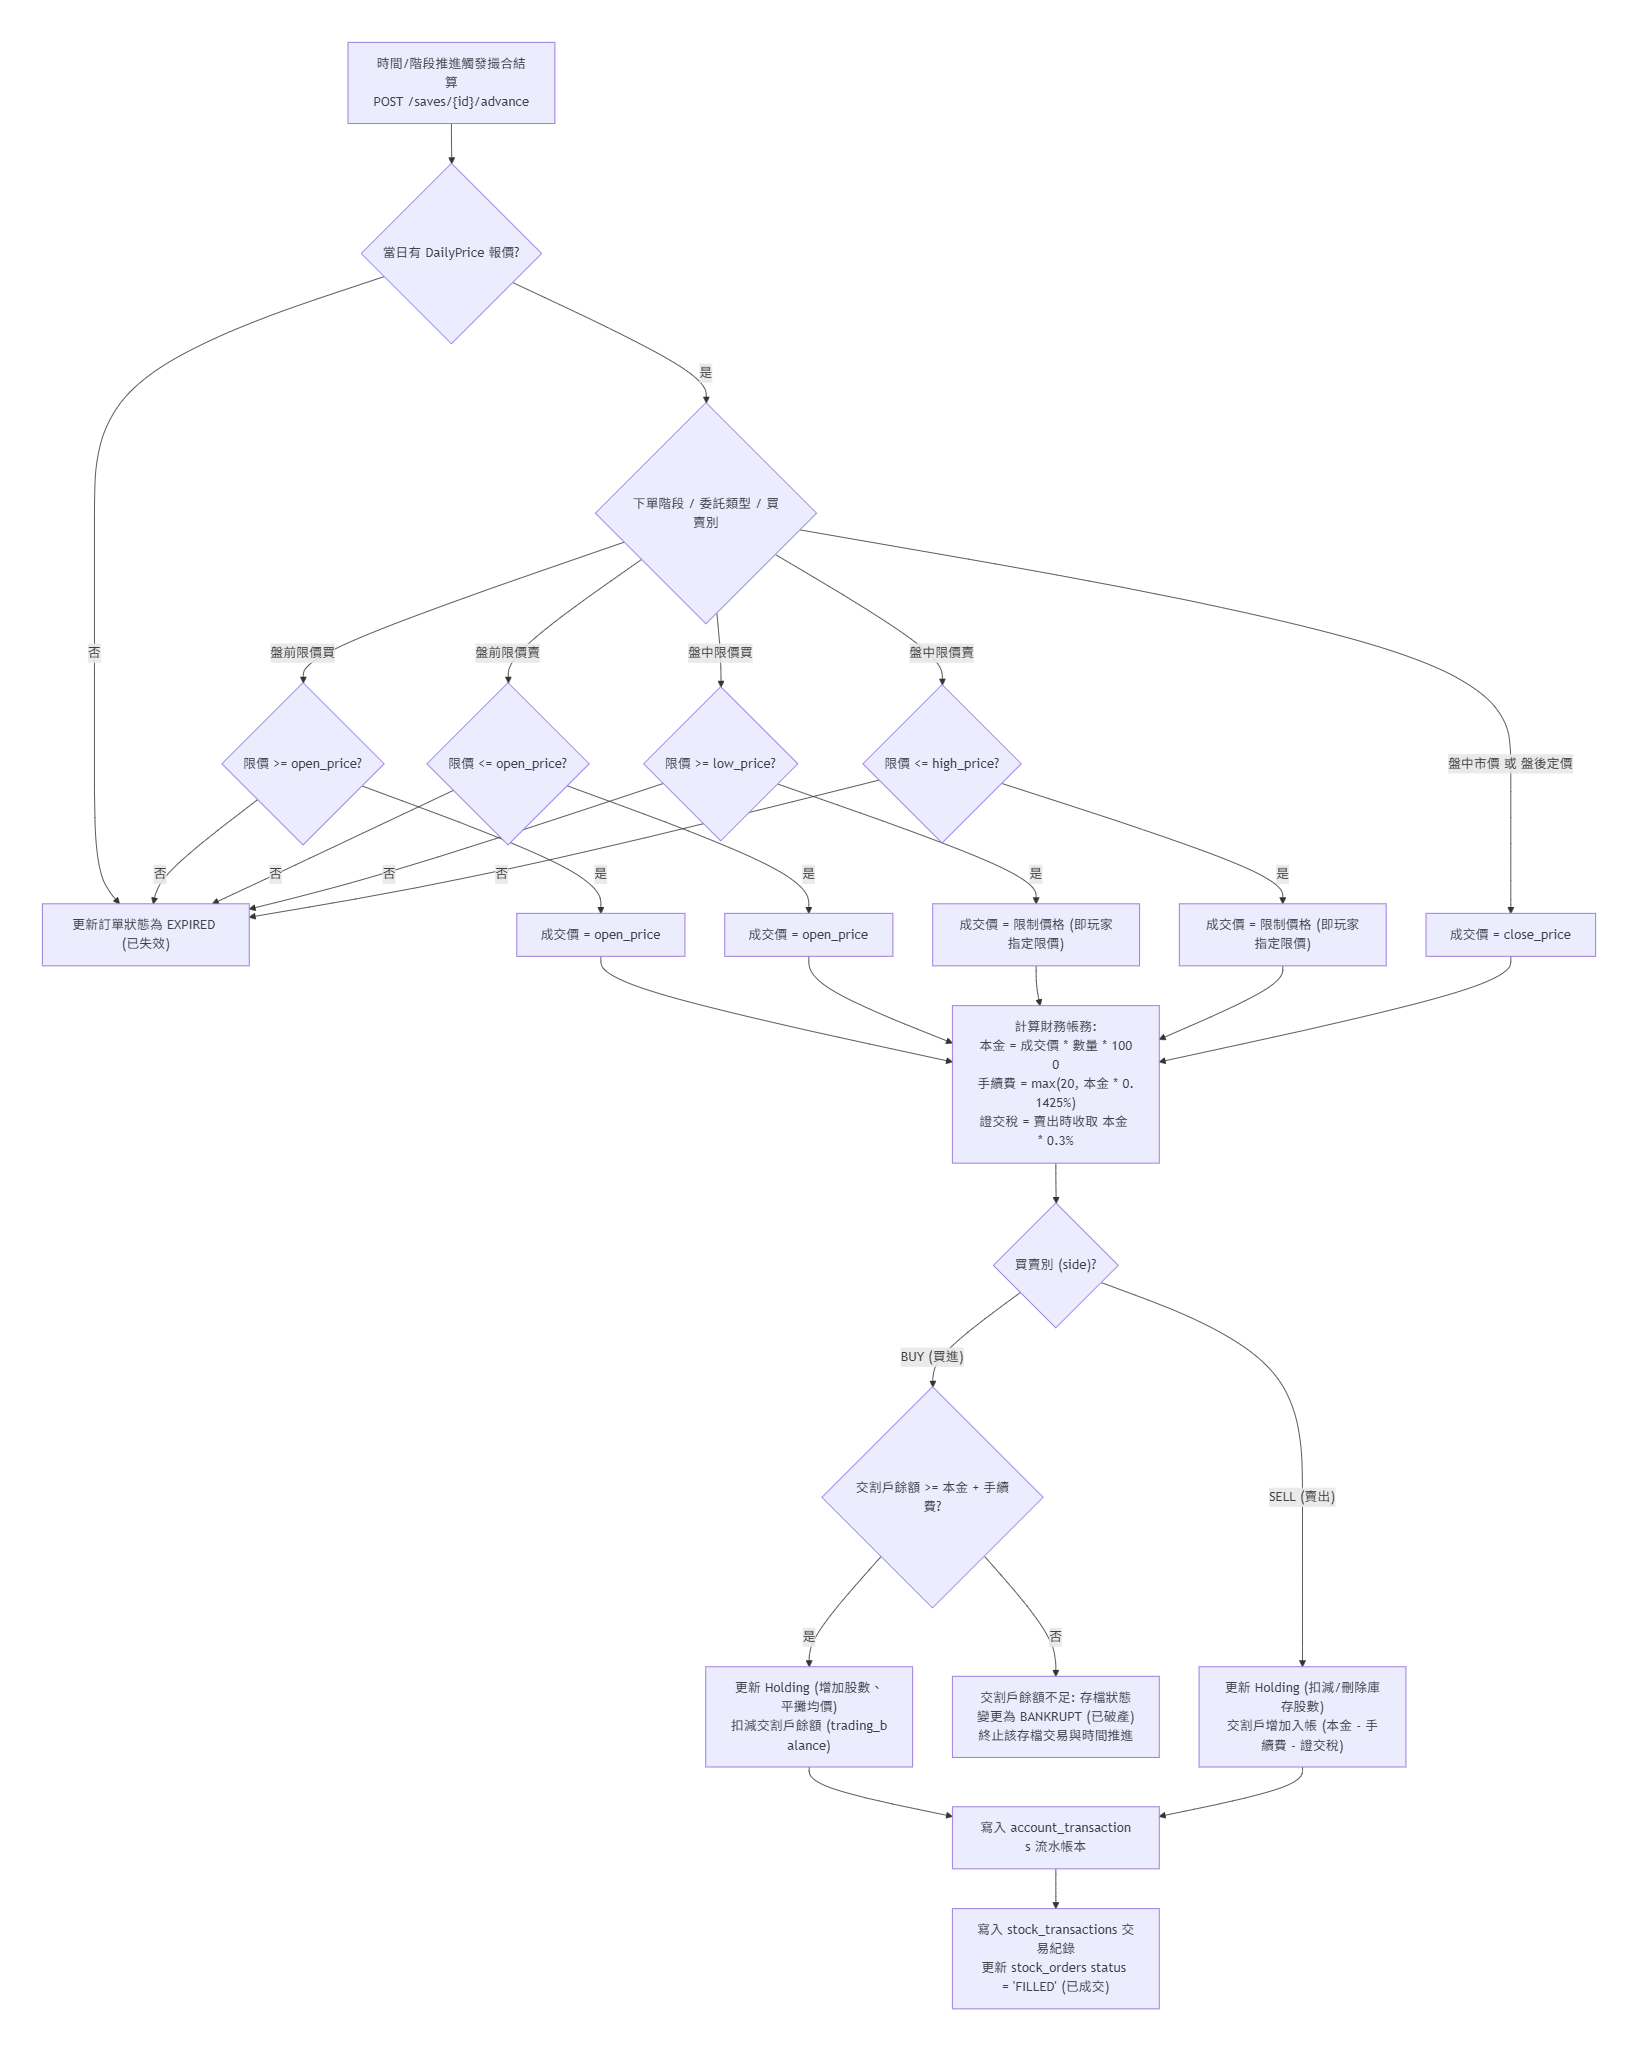
\includegraphics[width=0.99\textwidth]{flowchart/7_2_stock_transact.png}
        \caption{交易撮合流程圖}
    \end{figure}

    \subsection{介面設計}
    本系統的前端使用者介面（User Interface）採用現代暗色系（Dark Mode）風格設計，以簡潔直觀的卡片式佈局與豐富的色彩警示（如漲跌紅綠色標記）提升操作體驗。以下為系統之七個核心畫面設計：

    \begin{enumerate}
        \item \textbf{登入與註冊畫面} \\
        登入與註冊頁面為獨立的單一卡片式介面。登入畫面（Figure~\ref{fig:ui_login}）包含使用者帳號與密碼輸入框，並設有即時欄位格式與錯誤驗證提示（如紅字「錯誤訊息在這裡」），下方提供「Login」按鈕及引導至註冊頁面的連結；註冊畫面（Figure~\ref{fig:ui_signup}）則為對稱設計之帳號創建介面。

        \begin{figure}[H]
            \centering
            \begin{minipage}{0.48\textwidth}
                \centering
                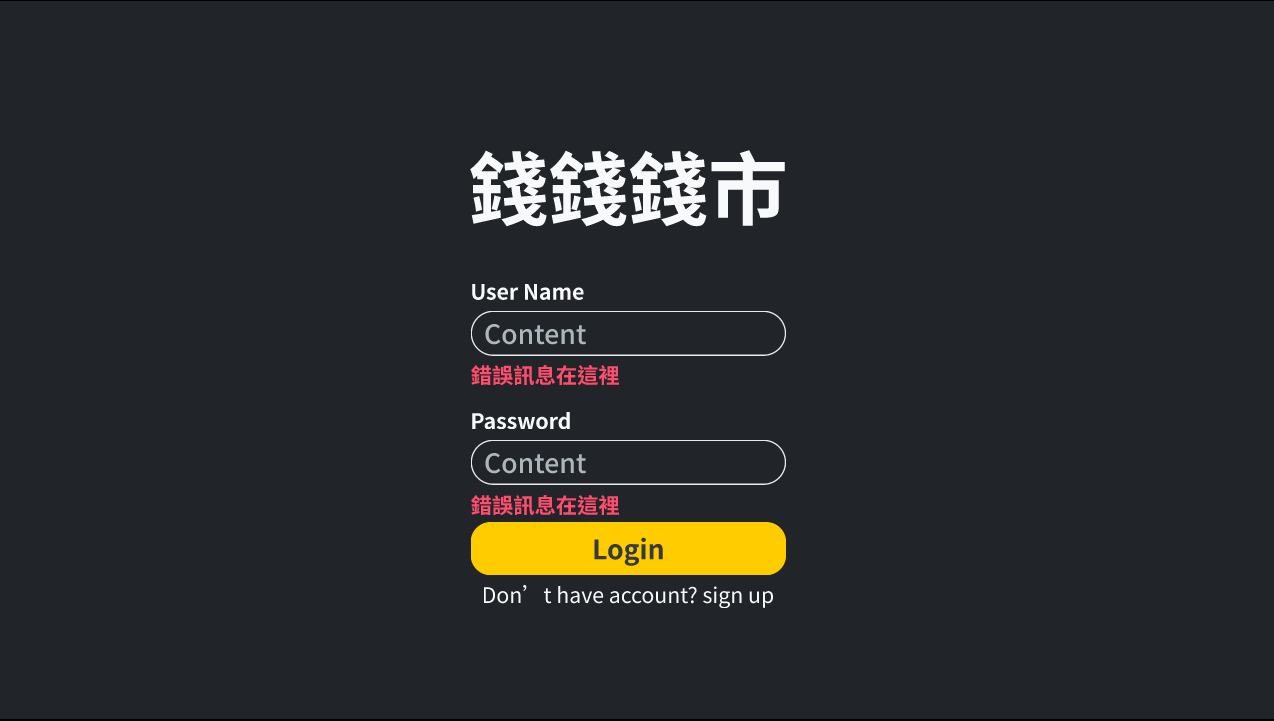
\includegraphics[width=\textwidth]{frontend_design/1_login.png}
                \caption{登入畫面設計}
                \label{fig:ui_login}
            \end{minipage}
            \hfill
            \begin{minipage}{0.48\textwidth}
                \centering
                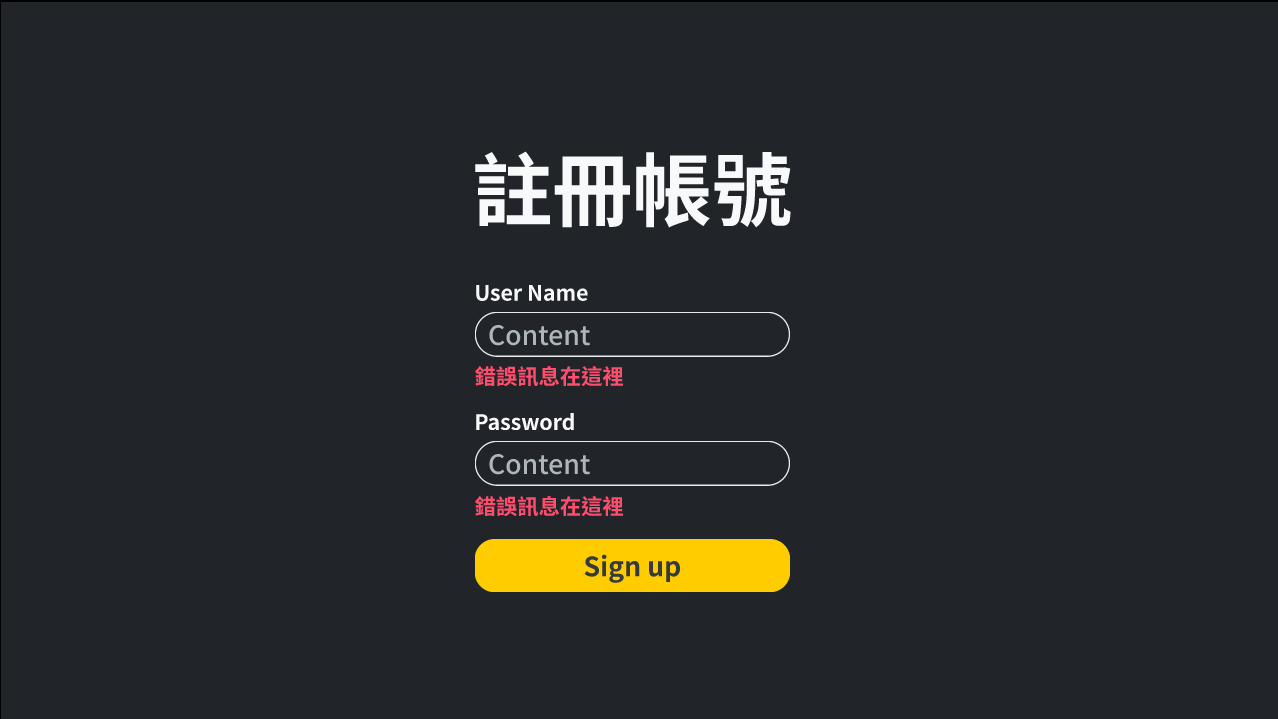
\includegraphics[width=\textwidth]{frontend_design/2_signup.png}
                \caption{註冊畫面設計}
                \label{fig:ui_signup}
            \end{minipage}
        \end{figure}

        \item \textbf{存檔列表與載入畫面} \\
        以彈出式對話框（Figure~\ref{fig:ui_select_savefile}）展示當前帳號名下的所有模擬存檔，以表格列出各存檔的虛擬時間、帳戶總資產、歷史報酬率、進行狀態與備註，上方設有黃色新增存檔按鈕（\texttt{+}）與粉紅色刪除存檔按鈕（\texttt{x}）以便於管理。

        \item \textbf{自選觀察清單畫面} \\
        系統主控制中心（Figure~\ref{fig:ui_watchlist}），左上角狀態列顯示虛擬日期與時間階段，右上角則即時更新存款戶與交割戶之餘額。自選股清單中展示代碼、名稱、當前股價、漲跌金額與漲跌幅（以紅字與綠字標註漲跌）；上方設有黃色按鈕（\texttt{+}）以搜尋並新增自選股，以及綠色的推進時間按鈕（\texttt{箭頭}）以推進交易階段。
        選擇自選股則會跳出該股票的詳細資訊卡片（Figure~\ref{fig:ui_stock_detail}）。
        \begin{figure}[H]
            \centering
            \begin{minipage}{0.48\textwidth}
                \centering
                
\includegraphics[width=\textwidth]{frontend_design/3_select_savefile.png}
                \caption{存檔紀錄視窗設計}
                \label{fig:ui_select_savefile}
            \end{minipage}
            \hfill
            \begin{minipage}{0.48\textwidth}
                \centering
                
\includegraphics[width=\textwidth]{frontend_design/4_watchlist.png}
                \caption{自選股主畫面設計}
                \label{fig:ui_watchlist}
            \end{minipage}
        \end{figure}

        \begin{figure}[H]
            \centering
            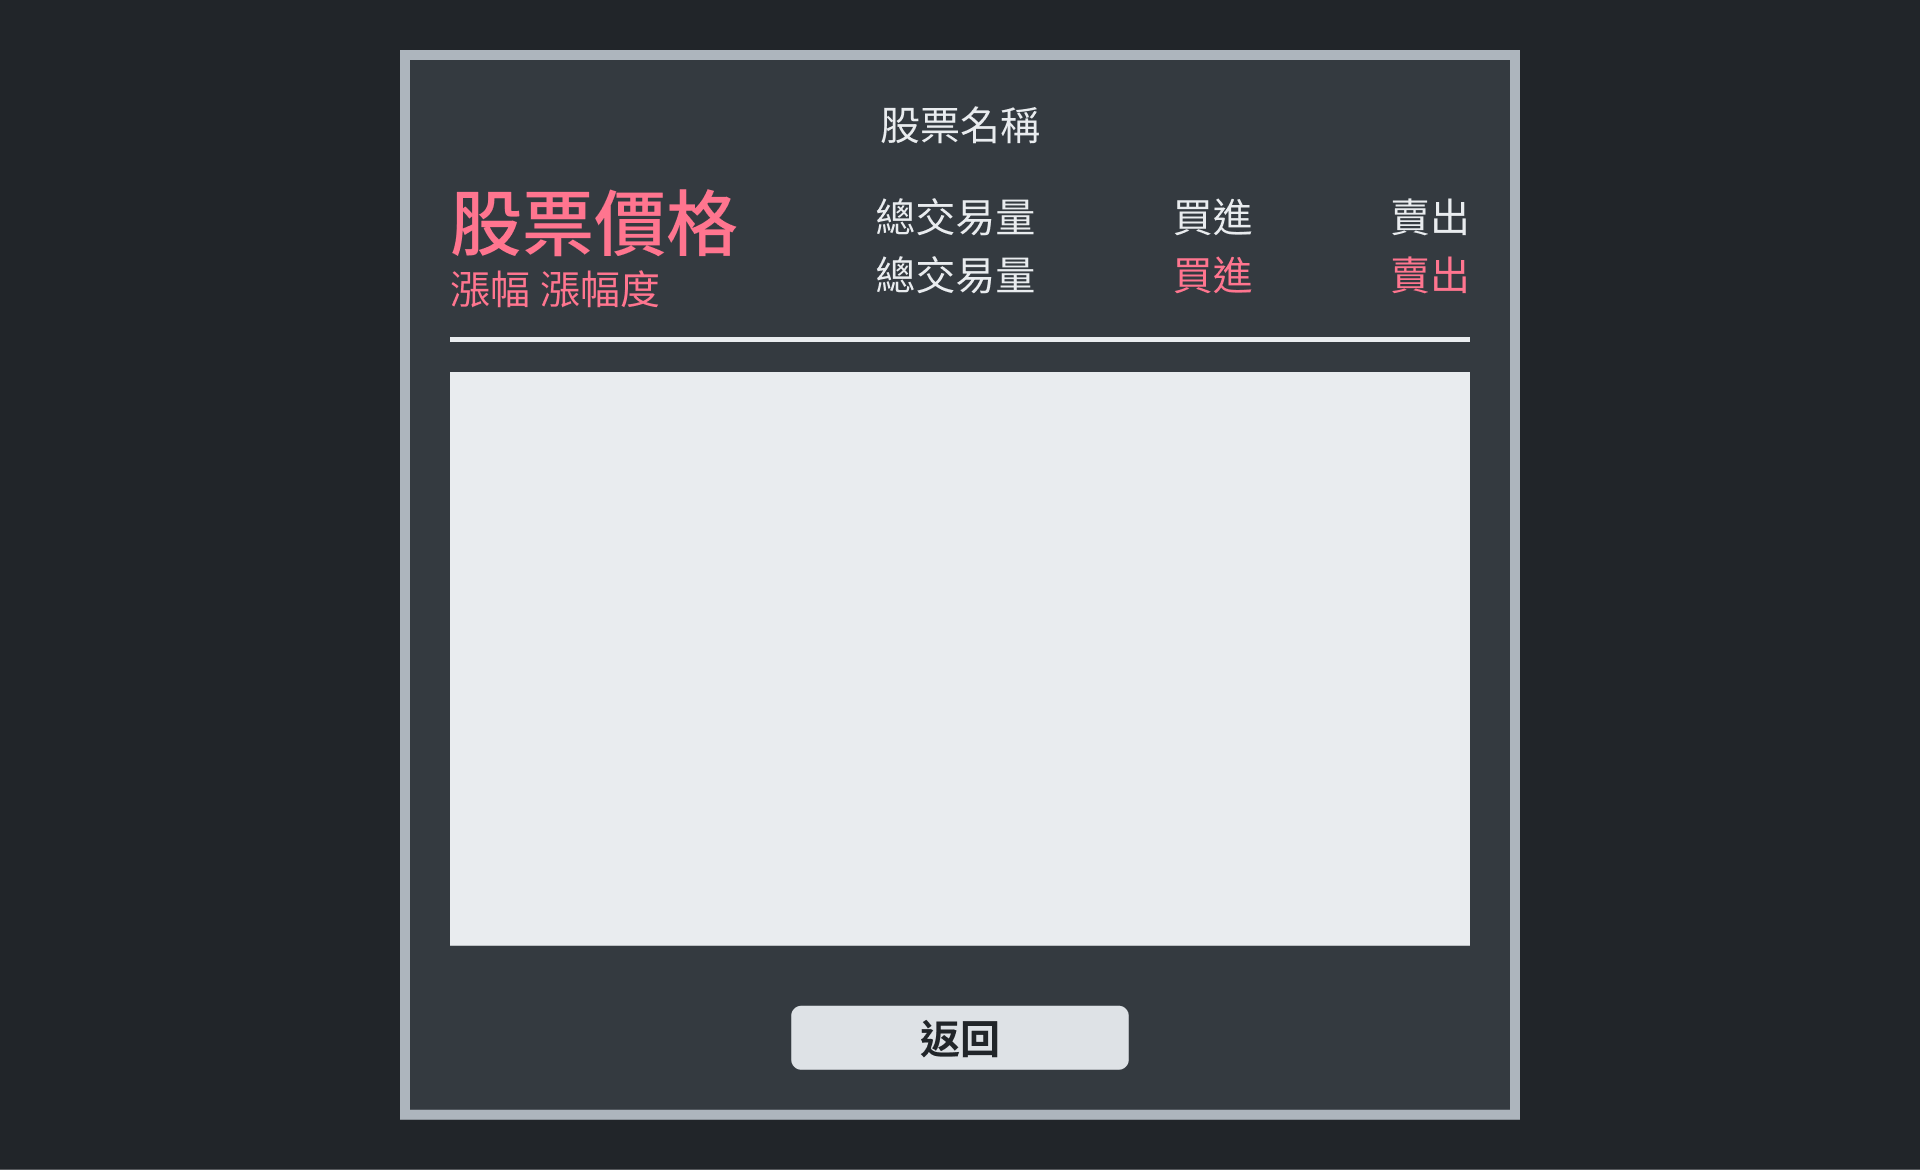
\includegraphics[width=0.6\textwidth]{frontend_design/4_1_stock_detail.png}
            \caption{股票詳細資訊卡片設計}
            \label{fig:ui_stock_detail}
        \end{figure}

        \item \textbf{下單交易委託畫面} \\
        在「交易」分頁下（Figure~\ref{fig:ui_order}），玩家可進行股票下單。左側填入股票代碼、委託價格及張數，設有防呆錯誤提示；右側設有兩個切換開關（Switch），上開關可切換「買/賣」，下開關可切換「限價/市價」，介面設計精簡防呆。

        \item \textbf{持股庫存與銀行轉帳畫面} \\
        在「庫存」分頁下（Figure~\ref{fig:ui_holding}），上半部為銀行帳本互轉介面，直觀展示交割戶與存款戶的金額，點擊中央雙向箭頭即可將款項互轉（Figure~\ref{fig:ui_transfer}）；下半部則顯示持股明細表，列出代碼、名稱、庫存張數、原幣損益、獲利率、現價與加權平均成本，並加總顯示總未實現損益。

        \begin{figure}[H]
            \centering
            \begin{minipage}{0.48\textwidth}
                \centering
                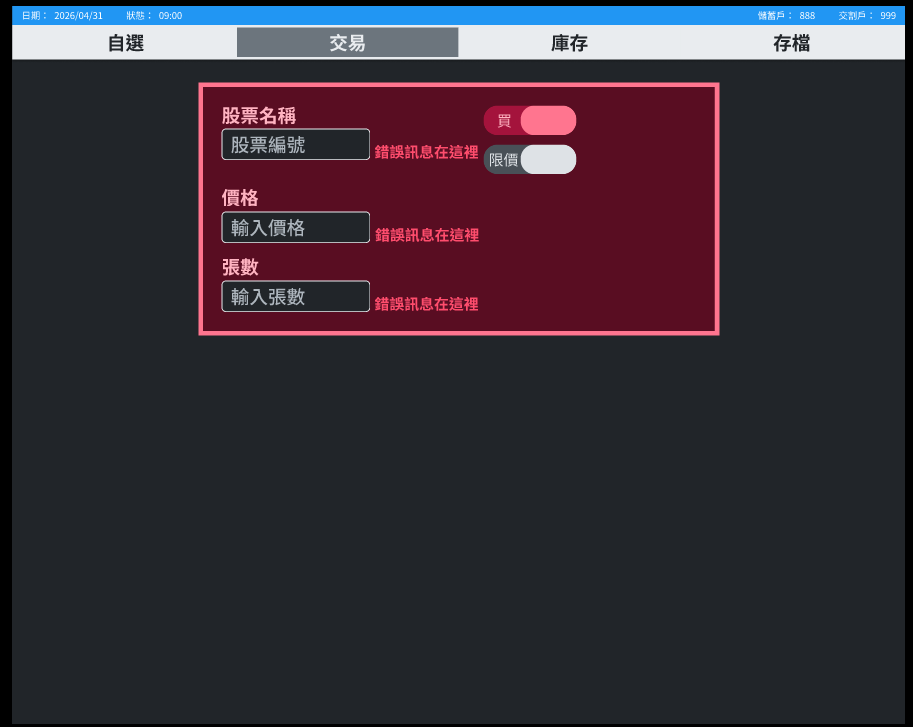
\includegraphics[width=\textwidth]{frontend_design/5_order.png}
                \caption{下單委託畫面設計}
                \label{fig:ui_order}
            \end{minipage}
            \hfill
            \begin{minipage}{0.48\textwidth}
                \centering
                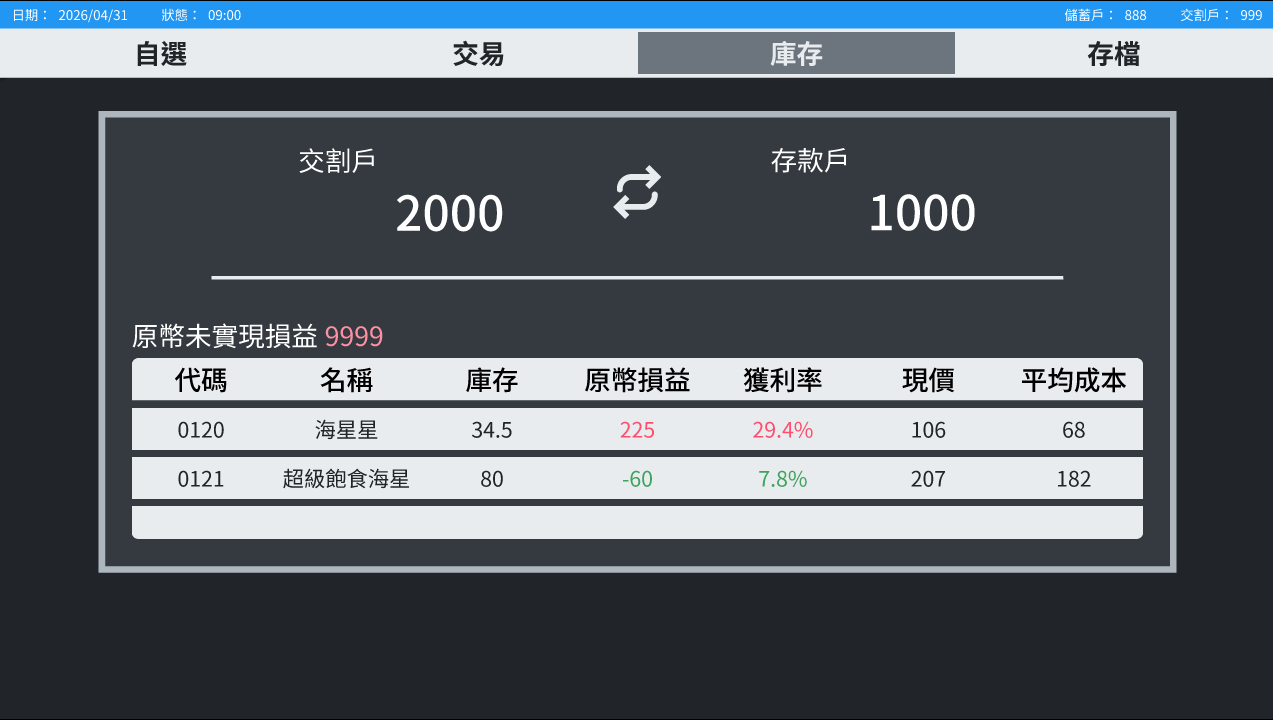
\includegraphics[width=\textwidth]{frontend_design/6_holding.png}
                \caption{資產庫存畫面設計}
                \label{fig:ui_holding}
            \end{minipage}
        \end{figure}

        \begin{figure}[H]
            \centering
            
\includegraphics[width=0.6\textwidth]{frontend_design/6_1_transfer.png}
            \caption{轉帳畫面設計}
            \label{fig:ui_transfer}
        \end{figure}
        \item \textbf{歷史紀錄與存檔紀錄分頁} \\
        在「存檔」分頁下（Figure~\ref{fig:ui_history}），左側顯示當前存檔的出帳投資總額、已實現損益與整體投資報酬率；右上角提供下拉式選單（交易紀錄、轉帳紀錄、存檔紀錄），下方則配合選單切換展示對應的歷次股票成交明細或資金異動流水帳，落實全面對帳之功能。
        \begin{figure}[H]
            \centering
            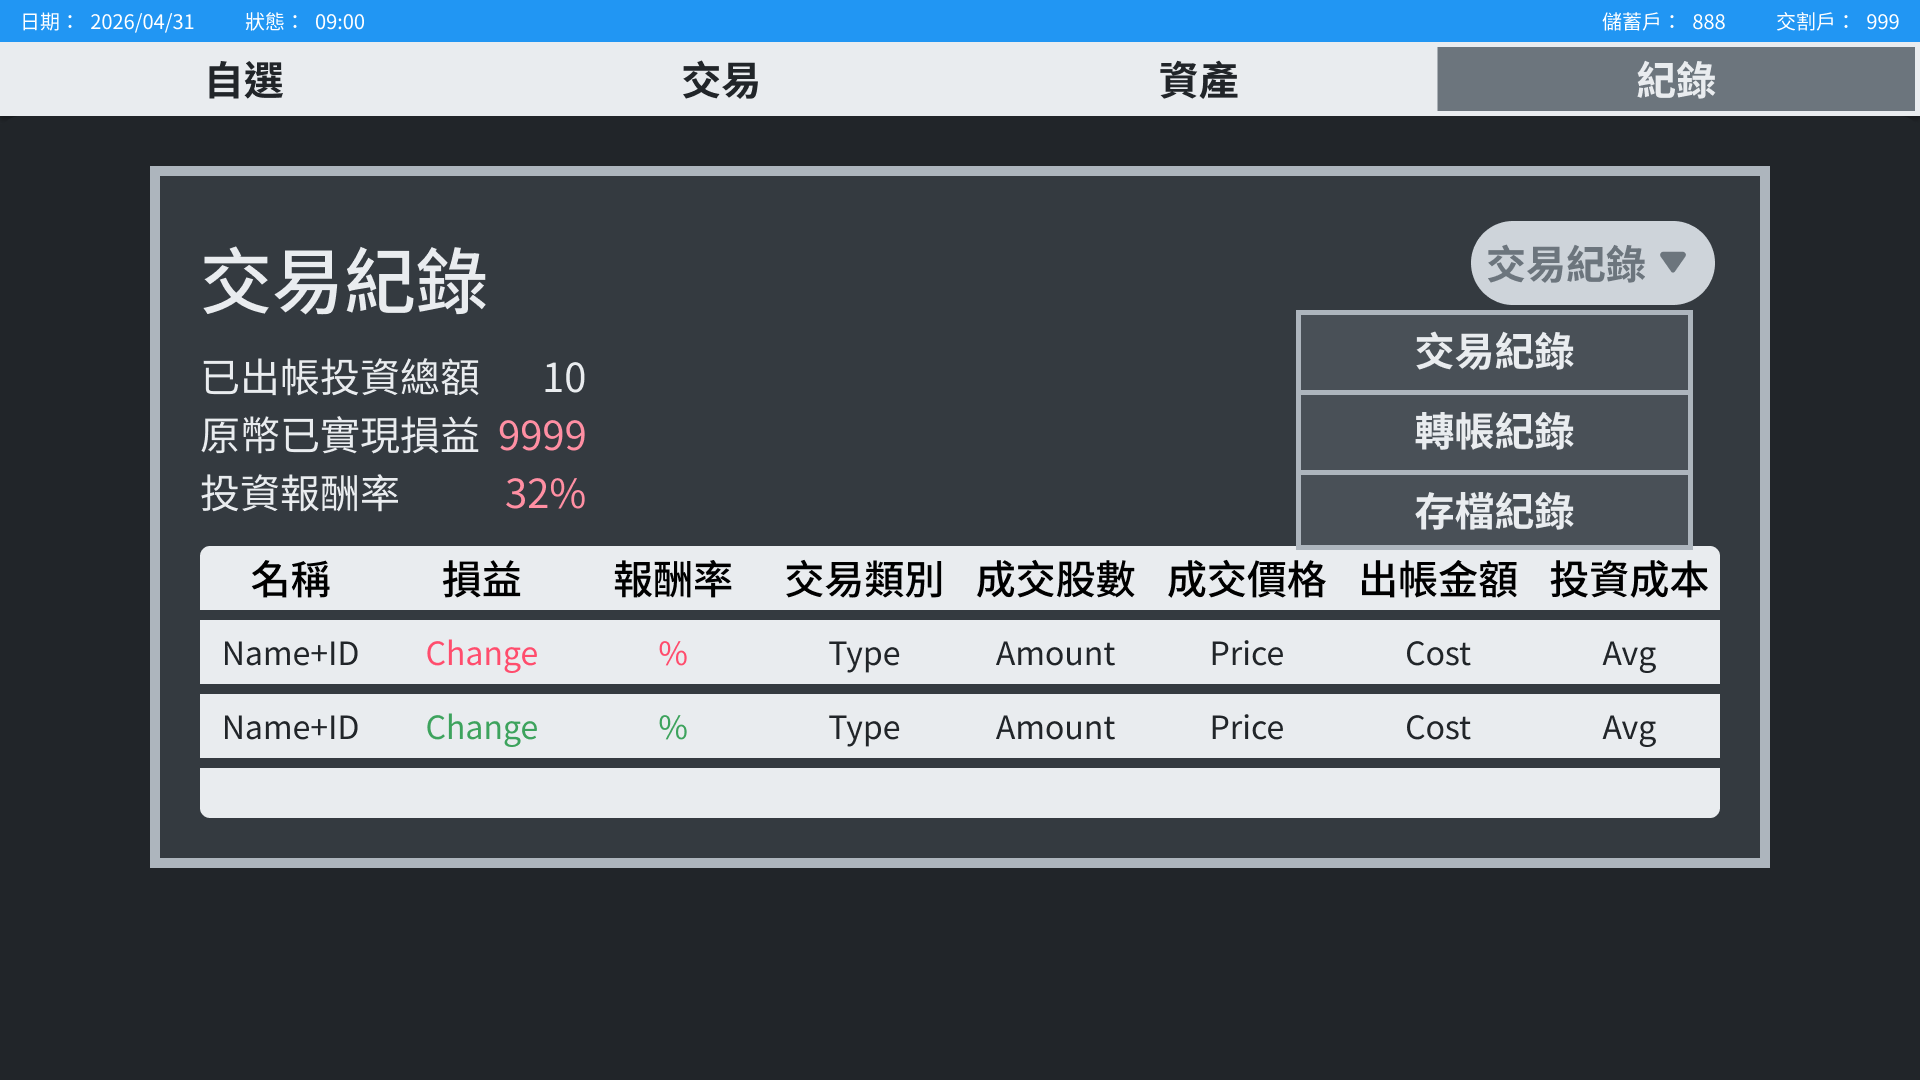
\includegraphics[width=0.6\textwidth]{frontend_design/7_transact.png}
            \caption{歷史明細紀錄畫面設計}
            \label{fig:ui_history}
        \end{figure}
    \end{enumerate}
    \subsection{連結資料庫部份之技術}
    \subsubsection{資料庫部署}
    本系統使用 MySQL 8.0 作為關聯式資料庫，以 Docker 容器化方式部署於遠端伺服器。
    資料目錄掛載至主機路徑，確保容器重啟或重建後資料持久保存。
    MySQL 容器僅存在於 Docker 內部網路，不對外直接暴露 port，從網路層隔離外部直連風險。

    \subsubsection{存取架構}
    應用層不直接連接 MySQL，而是透過自行建置的 HTTP SQL API（Node.js）作為唯一存取入口：
    \[
    \text{應用程式} \to \text{HTTP POST} \to \text{SQL API (Node.js)} \to \text{MySQL 8.0}
    \]
    SQL API 接收 JSON 格式的 SQL 語句後執行並回傳結果，所有外部存取皆須經過此中間層，統一管控資料庫操作。

    \subsubsection{遠端安全存取}
後端與資料匯入工具部署於不同主機，透過 Tailscale（基於 WireGuard 協定的零信任私有網路）建立加密隧道，以私有域名（sql-api.shiragaserver.lan）存取 SQL API，無需開放公網 port。

    \subsubsection{資料匯入}
    歷史股票資料（TEJ 原始 CSV）經專用清理腳本處理後，以批次 INSERT ... ON DUPLICATE KEY UPDATE 方式寫入，兼顧初次匯入與後續更新的冪等性。

    \subsubsection{自動備份}
    搭配 mysql-cron-backup 服務，每日凌晨 02:00 自動執行 mysqldump，保留最近 5 份，存放於主機本地目錄。

    \begin{figure}[H]
        \centering
        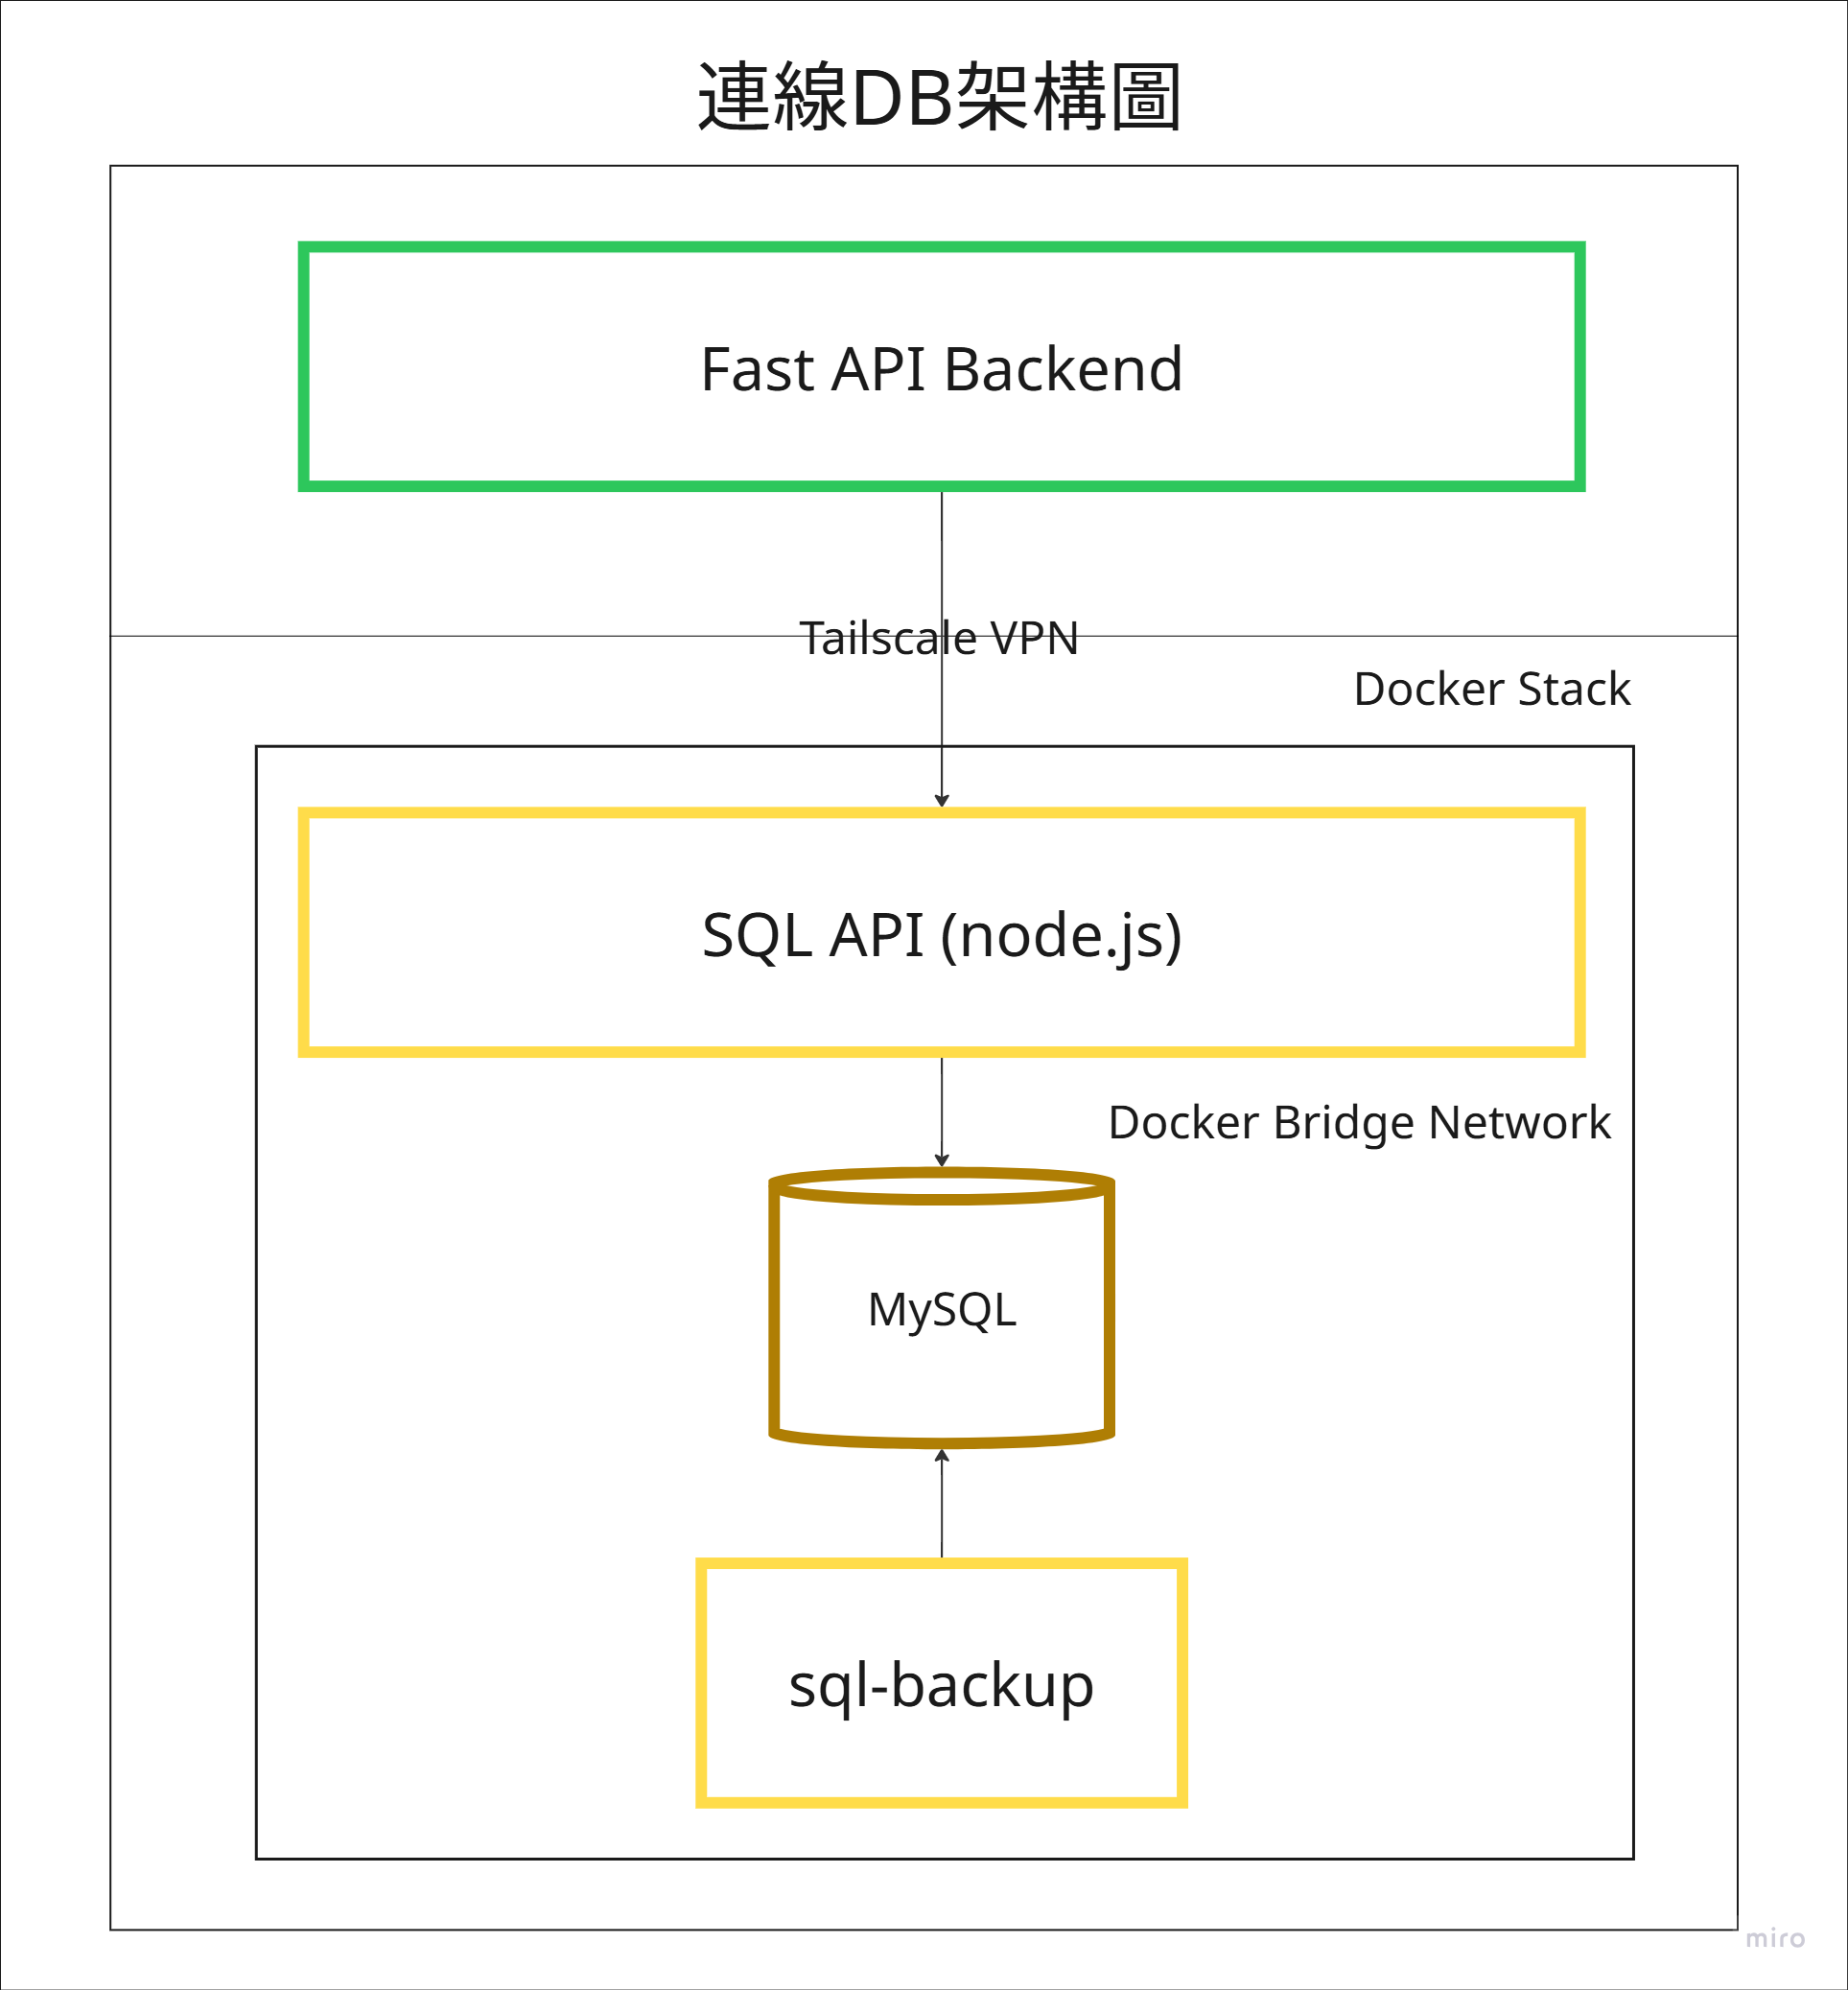
\includegraphics[width=0.6\textwidth]{flowchart/11_db.png}
        \caption{資料庫存取架構圖}
        \label{fig:db_architecture}
    \end{figure}
    \section{預定工作分配}
    本組期末專案開發之預定工作分配如下：
    \begin{center}
    \begin{tabular}{|l|l|p{8cm}|}
    \hline
    \textbf{組員} & \textbf{學號} & \textbf{負責項目} \\
    \hline
    楊凱臣 & 41347001S & 系統架構設計、核心業務邏輯規劃、前端 K 線圖設計、後端 FastAPI 開發 \\ \hline
    周聖詠 & 41347009S & 後端 FastAPI 開發 \\ \hline
    許育綸 & 41347011S & 前端介面設計與 Vue.js 開發 \\ \hline
    盧人豪 & 41347041S & 後端 FastAPI 開發與伺服器維護 \\ \hline
    \end{tabular}
    \end{center}
\appendix
\section{附錄：Report 1}

\includepdf[
    pages={-}, 
    pagecommand={\thispagestyle{headings}}, 
    scale=0.99, 
    offset=0 -0cm % 調整 PDF 位置以避免蓋住標題
]{../report1-2/report1-2.pdf}

\newpage
\section{附錄：Report 2 E-R Diagram}
\label{sec:appendix_er}
{
\begin{center}
    
\resizebox{\textwidth}{!}{ 
    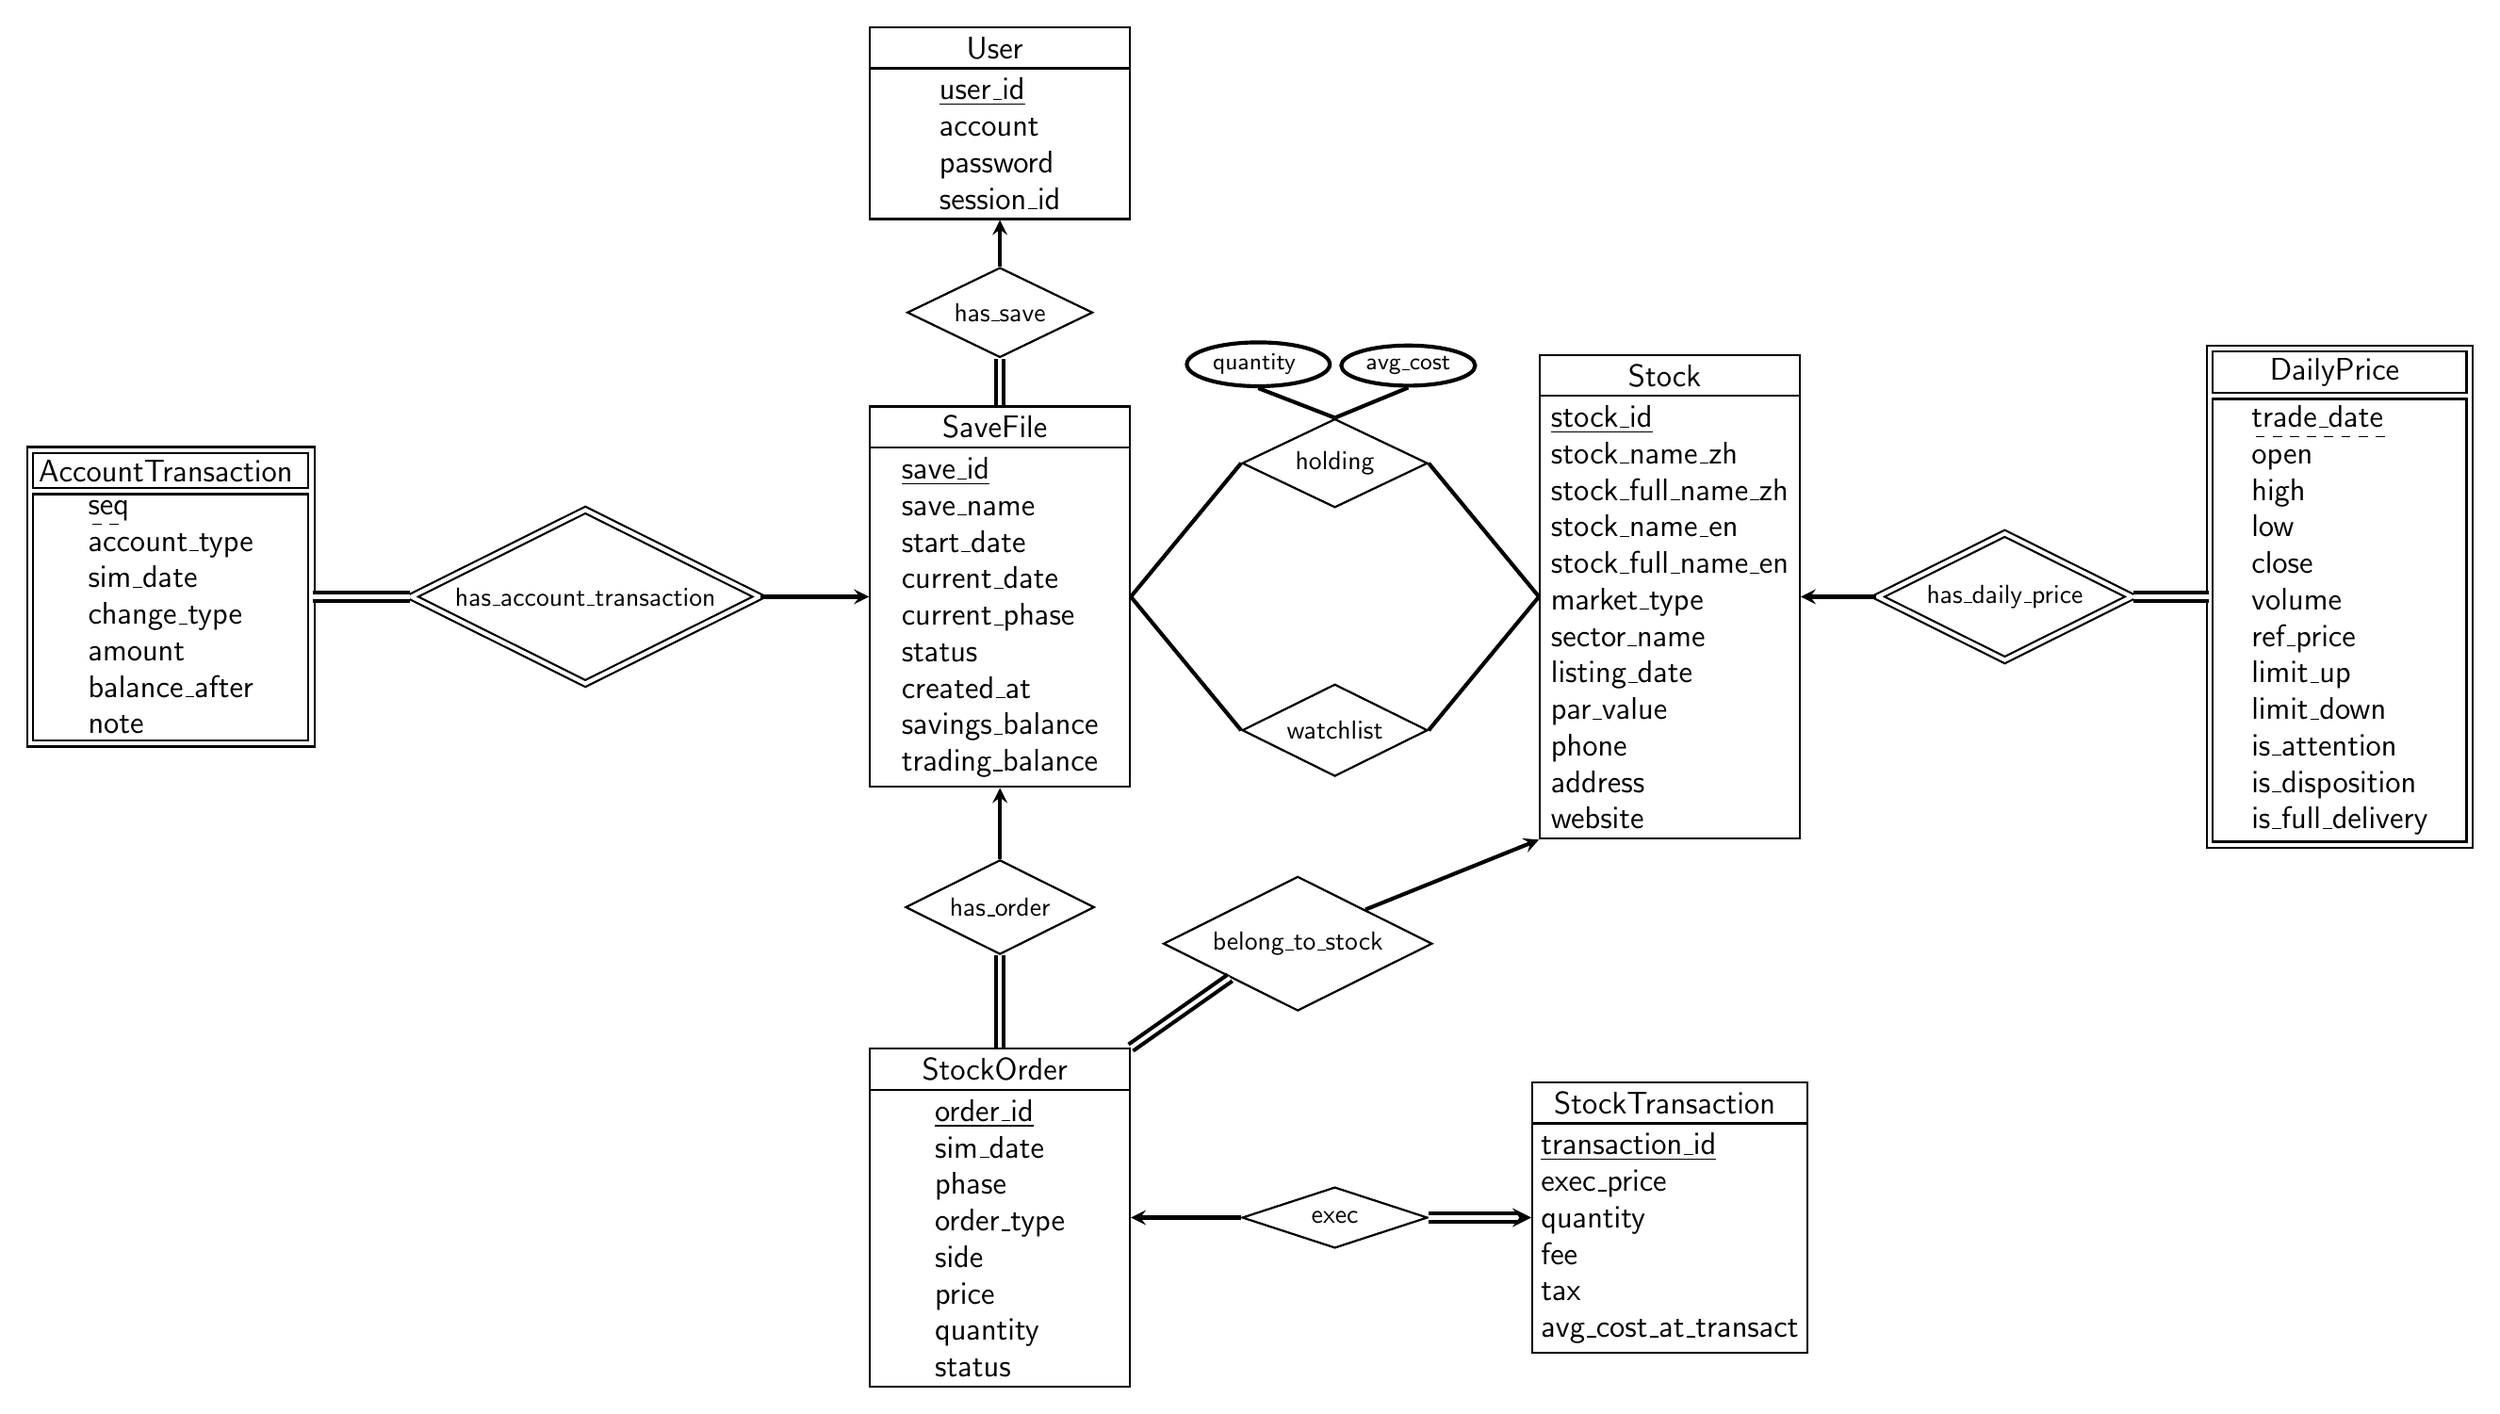
\begin{tikzpicture}[
        >=stealth,
        % 線條樣式
        every path/.style={line width=1.5pt},
        % 實體樣式 (單線方框)
        entity/.style={
            rectangle split, rectangle split parts=2,
            draw, thick, align=left, minimum width=3.5cm, font=\sffamily\large
        },
        % 弱實體樣式 (雙線方框)
        weakentity/.style={
            rectangle split, rectangle split parts=2,
            draw, thick, double, double distance=1.5pt, align=left, minimum width=3.5cm, font=\sffamily\large
        },
        % 關聯樣式 (單線菱形)
        relationship/.style={
            diamond, draw, thick, aspect=2, minimum width=2.5cm, align=center, font=\sffamily
        },
        % 弱關聯樣式 (雙線菱形)
        weakrel/.style={
            diamond, draw, thick, double, double distance=1.5pt, aspect=2, minimum width=2.5cm, align=center, font=\sffamily
        },
        % 屬性樣式
        attribute/.style={
            ellipse, draw, align=center, font=\sffamily\small, inner sep=2pt
        },
        % 連線樣式 (全參與/雙線)
        total/.style={double, double distance=1.5pt} 
    ]

        % ==========================
        % 1. 建立實體 (Entities)
        % ==========================
        
        % SaveFile (中心)
        \node[entity] (savefile) {
            \hfil SaveFile \hfil 
            \nodepart{two} 
            \underline{save\_id} \\ save\_name \\ start\_date \\ current\_date \\ 
            current\_phase \\ status \\ created\_at \\ savings\_balance \\ trading\_balance
        };

        % User (上)
        \node[entity] (user) [above=2.5cm of savefile] {
            \hfil User \hfil 
            \nodepart{two} 
            \underline{user\_id} \\ account \\ password \\ session\_id
        };

        % AccountTransaction (左) - 弱實體
        \node[weakentity] (acctrans) [left=7.5cm of savefile] {
            \hfil AccountTransaction \hfil 
            \nodepart{two} 
            \dashuline{seq} \\ account\_type \\ sim\_date \\ 
            change\_type \\ amount \\ balance\_after \\ note
        };

        % Stock (右)
        \node[entity] (stock) [right=5.5cm of savefile] {
            \hfil Stock \hfil 
            \nodepart{two} 
            \underline{stock\_id} \\ stock\_name\_zh \\ stock\_full\_name\_zh \\ stock\_name\_en \\
            stock\_full\_name\_en \\ market\_type  \\ sector\_name  \\ 
            listing\_date \\ par\_value  \\ phone  \\ 
            address \\ website 
        };

        % DailyPrice (最右) - 弱實體
        \node[weakentity] (dailyprice) [right=5.5cm of stock] {
            \hfil DailyPrice \hfil 
            \nodepart{two} 
            \dashuline{trade\_date} \\ open \\ high \\ low \\ close \\ 
            volume \\ ref\_price \\ limit\_up \\ 
            limit\_down \\ is\_attention \\ 
            is\_disposition \\ is\_full\_delivery 
        };

        % StockOrder (下)
        \node[entity] (stockorder) [below=3.5cm of savefile] {
            \hfil StockOrder \hfil 
            \nodepart{two} 
            \underline{order\_id} \\ sim\_date \\ phase \\ 
            order\_type  \\ side \\ price \\ 
            quantity  \\ status
        };

        % StockTransaction (StockOrder的右側，Stock的正下方)
        \node[entity] (stocktrans) at (stock |- stockorder) {
            \hfil StockTransaction \hfil 
            \nodepart{two} 
            \underline{transaction\_id} \\ exec\_price \\ 
            quantity  \\ fee  \\ tax \\ 
            avg\_cost\_at\_transact
        };

        % ==========================
        % 2. 建立關聯與連線
        % ==========================

        % User <-> SaveFile 
        \node[relationship] (hassave) at ($(user)!0.4!(savefile)$) {has\_save};
        \draw[<-] (user.south) -- (hassave.north);
        \draw[total] (savefile.north) -- (hassave.south);

        % SaveFile <-> AccountTransaction (弱關聯)
        \node[weakrel] (hasacctrans) at ($(savefile)!0.5!(acctrans)$) {has\_account\_transaction};
        \draw[<-] (savefile.west) -- (hasacctrans.east);
        \draw[total] (hasacctrans.west) -- (acctrans.east);

        % SaveFile <-> Stock (Holding & Watchlist)
        \path (savefile.east) -- (stock.west) coordinate[midway] (mid_ss);
        \node[relationship] (holding) at ($(mid_ss) + (0, 1.8)$) {holding};
        \node[relationship] (watchlist) at ($(mid_ss) + (0, -1.8)$) {watchlist};

        \draw (savefile.east) -- (holding.west);
        \draw (savefile.east) -- (watchlist.west);
        \draw (holding.east) -- (stock.west);
        \draw (watchlist.east) -- (stock.west);

        % Holding 屬性
        \node[attribute] (qty) [above left=0.8cm and -0.3cm of holding] {quantity };
        \node[attribute] (avgcost) [above right=0.8cm and -0.3cm of holding] {avg\_cost};
        \draw (holding.north) -- (qty.south);
        \draw (holding.north) -- (avgcost.south);

        % Stock <-> DailyPrice (弱關聯)
        \node[weakrel] (hasdailyprice) at ($(stock)!0.5!(dailyprice)$) {has\_daily\_price};
        \draw[<-] (stock.east) -- (hasdailyprice.west);
        \draw[total] (hasdailyprice.east) -- (dailyprice.west);

        % SaveFile <-> StockOrder
        \node[relationship] (hasorder) at ($(savefile)!0.5!(stockorder)$) {has\_order};
        \draw[<-] (savefile.south) -- (hasorder.north);
        \draw[total] (hasorder.south) -- (stockorder.north);

        % StockOrder <-> StockTransaction (exec)
        \node[relationship] (exec) at ($(stockorder)!0.5!(stocktrans)$) {exec};
        \draw[<-] (stockorder.east) -- (exec.west);
        \draw[total,->] (exec.east) -- (stocktrans.west);

        % StockOrder <-> Stock (belong_to_stock)
        % 將菱形置於兩者連線的中間偏左上角，避免線條與其他實體重疊
        \node[relationship] (belongto) at ($(stockorder.north east)!0.5!(stock.south west) + (-0.5, 0)$) {belong\_to\_stock};
        \draw[total] (stockorder.north east) -- (belongto.south west);
        \draw[<-] (stock.south west) -- (belongto.north east);

    \end{tikzpicture}
}
\end{center}
}

\end{document}